\documentclass[a4paper,reqno,10pt]{amsart}
\usepackage{a4wide}
\usepackage{amsmath,amssymb,amsfonts,amsthm,mathtools}
\usepackage{amscd}
\usepackage{tikz-cd}
\usetikzlibrary{arrows.meta,positioning}
\usepackage{enumitem}
\usepackage{microtype}
\usepackage[colorlinks=true,linkcolor=blue,citecolor=blue,urlcolor=blue]{hyperref}
\setlist[enumerate]{leftmargin=*}
\setlist[enumerate,1]{label={\upshape(\arabic*)}}
\setlist[enumerate,2]{label={\upshape(\alph*)}}
\newtheorem{theorem}{Theorem}[section]
\newtheorem{proposition}[theorem]{Proposition}
\newtheorem{lemma}[theorem]{Lemma}
\newtheorem{corollary}[theorem]{Corollary}
\newtheorem*{theoremA}{Theorem A}
\theoremstyle{definition}
\newtheorem{definition}[theorem]{Definition}
\newtheorem{setting}[theorem]{Setting}
\newtheorem{construction}[theorem]{Construction}
\newtheorem{example}[theorem]{Example}
\newtheorem{remark}[theorem]{Remark}
\newtheorem*{organization}{Organization}
\newtheorem*{conventions}{Conventions and notation}
\newtheorem*{aiuse}{Use of AI}
\numberwithin{equation}{section}
\DeclareMathOperator{\moduleCategory}{\mathsf{mod}}
\renewcommand{\mod}{\moduleCategory}
\DeclareMathOperator{\ind}{ind}
\DeclareMathOperator{\add}{add}
\DeclareMathOperator{\Hom}{Hom}
\DeclareMathOperator{\Ext}{Ext}
\DeclareMathOperator{\End}{End}
\DeclareMathOperator{\Irr}{Irr}
\DeclareMathOperator{\rad}{rad}
\DeclareMathOperator{\soc}{soc}
\DeclareMathOperator{\supp}{supp}
\DeclareMathOperator{\ann}{ann}
\newcommand{\op}{\mathrm{op}}
\newcommand{\cC}{\mathcal C}
\newcommand{\cD}{\mathcal D}
\newcommand{\cH}{\mathcal H}
\newcommand{\cP}{\mathcal P}
\newcommand{\cV}{\mathcal V}
\newcommand{\cW}{\mathcal W}
\newcommand{\Abar}{\overline A}
\newcommand{\eps}{\varepsilon}
\newcommand{\one}{\mathbf 1}
\newcommand{\indicator}{\mathbf 1}
\newcommand{\spmod}{\mod_{\mathrm{sp}}}
\newcommand{\TSp}{T\text{-}\mathsf{Sp}}
\newcommand{\Dk}{D_k}
\newcommand{\indeg}{\operatorname{indeg}}
\newcommand{\outdeg}{\operatorname{outdeg}}
\newcommand{\uhom}{\underline{\Hom}}
\newcommand{\ohom}{\overline{\Hom}}

\title{The magnitude conjecture for module categories}
\author[H.\ Enomoto]{Haruhisa Enomoto}
\address{Parakeet Inc., Japan}
\email{haruhisa.enomoto.math@gmail.com}
\subjclass[2020]{16G10, 16G70}
\keywords{magnitude, representation-finite algebra, Auslander--Reiten quiver,
\(\tau\)-category, special biserial algebra, poset representations}
\date{\today}
\begin{document}
\begin{abstract}
For a finite-dimensional representation-finite algebra over an algebraically
closed field, the matrix of Hom dimensions between representatives of the
indecomposable modules is known to be invertible. The magnitude of the module category
is the sum of the entries of its inverse. We prove
that this magnitude is at least the number of isomorphism classes of simple modules,
with equality precisely for special biserial algebras. This establishes
the conjecture of B{\o}rve, Horiatakis, and Kalck. For representation-finite
representation-directed algebras, magnitude minus the number of simple modules
cannot increase upon taking the quotient by the ideal generated by a
primitive idempotent. The proof combines Ringel--Vossieck's hammock theory,
through its description of certain quotient categories as categories of poset
representations, with a comparison of almost split sequences. We give direct
proofs of the required hammock-theoretic results in an appendix. For general
algebras, we reduce to the directed case using finite-dimensional algebras
constructed from graded modules.
\end{abstract}
\maketitle
\tableofcontents

\section{Introduction}\label{sec:introduction}
Let \(A\) be a finite-dimensional representation-finite algebra over an
algebraically closed field \(k\). Let \(\ind A\) be a set of
representatives of its indecomposable right modules, and fix an ordering of this set.
The Hom matrix
\[
 H_A=\bigl(\dim_k\Hom_A(X,Y)\bigr)_{X,Y\in\ind A}
\]
is invertible \cite[Lemma~1.9]{BHK}. B{\o}rve, Horiatakis, and Kalck
define the \emph{magnitude}
of the category \(\mod A\) of finite-dimensional right \(A\)-modules by
\[
 \chi(\mod A)=\one^{\mathsf T}H_A^{-1}\one,
\]
where \(\one\) is the column vector whose entries are all one
\cite[Definitions~1.2 and~1.6]{BHK}. Thus magnitude is the
sum of the entries of the inverse Hom matrix. Reordering \(\ind A\)
simultaneously permutes the rows and columns of \(H_A\) and of
\(H_A^{-1}\), leaving this sum unchanged.
Magnitude is also invariant under \(k\)-linear Morita equivalence
(Lemma~\ref{lem:invariance}).

Write \(|A|\) for the number of isomorphism classes of simple modules and \(a(A)\)
for the number of arrows in the Auslander--Reiten quiver, with
\(\dim_k\Irr_A(X,Y)\) arrows from \(X\) to \(Y\). The formula
\begin{equation}\label{eq:intro-count}
 \chi(\mod A)=2|\ind A|-|A|-a(A)
\end{equation}
was proved in \cite[Lemma~1.9]{BHK} using almost split sequences.
B{\o}rve, Horiatakis, and Kalck also proved that
\(\chi(\mod A)=|A|\) for special biserial algebras
(see Definition~\ref{def:special-biserial}) \cite[Theorem~3.5]{BHK}.
They conjectured that \(\chi(\mod A)\geq|A|\) for every
representation-finite algebra, with equality precisely for special biserial
algebras \cite[Conjecture~A]{BHK}. We prove this conjecture.

\begin{theoremA}[= Theorem~\ref{thm:main}]\label{thm:intro-main}
Let \(A\) be a finite-dimensional representation-finite algebra over an
algebraically closed field. Write \(|A|\) for its number of isomorphism
classes of simple modules. Then the following hold.
\begin{enumerate}
\item \(\chi(\mod A)\geq |A|\).
\item \(\chi(\mod A)=|A|\) if and only if \(A\) is special biserial.
\end{enumerate}
\end{theoremA}

The proof begins with representation-directed algebras. We show
that the \emph{magnitude surplus} \(\sigma(A)=\chi(\mod A)-|A|\) satisfies
\[
 \sigma(A)\geq\sigma(A/AeA)
\]
for every primitive idempotent \(e\). The quotient remains
representation-finite and representation-directed, since its module category
is a full subcategory of \(\mod A\). Successive deletions end at the zero
algebra, whose surplus is zero, and hence prove nonnegativity. A central step is an equivalence
between the additive quotient
\[
 (\mod A)/[\mod(A/AeA)]
\]
and a category of \emph{representations of a finite poset by subspaces}.
Here \(A/AeA\)-modules are regarded as \(A\)-modules annihilated by
\(e\), and brackets denote the ideal of maps factoring through them.
A representation of a poset by subspaces consists of a finite-dimensional
space \(V\) with subspaces \(V_t\), one for each poset element, such that
\(V_s\subseteq V_t\) when \(s\leq t\); morphisms preserve the specified
subspaces (Definition~\ref{def:t-space}). This equivalence is due to
Ringel--Vossieck \cite[Section~10, Theorem, p.~243]{RV}. Their hammock theory
relates the composition multiplicities of a fixed simple module to poset
representations and the lengths of paths in their Auslander--Reiten quivers.
We describe the poset and the equivalence explicitly in
Construction~\ref{con:poset} and Proposition~\ref{prop:poset-equivalence}.
Their path-length inequality \cite[Section~8, Proposition, p.~237]{RV}
says that every path from the unique source to the unique sink has length
at least the size of the poset. It gives the bound on the number of
irreducible arrows needed here. Iyama's quotient theorem
(Proposition~\ref{prop:quotient-sequences}) obtains the quotient's
\(\tau\)-sequences from almost split sequences by deleting the summands
annihilated by \(e\). These sequences generalize almost split sequences
to additive categories. We combine the arrow bound with a comparison of almost split
sequences over \(A\) and \(A/AeA\) (Proposition~\ref{prop:compensation})
to prove the deletion inequality \(\sigma(A)\geq\sigma(A/AeA)\).
Equality in this deletion inequality forces the simple module corresponding
to \(e\) to occur at most once as a composition factor of each indecomposable.

Appendix~\ref{app:structural} proves the structural statements used here
in their stated form, using the module and \(\tau\)-sequence preliminaries
of this paper. Thus these parts of the argument can be read without
consulting the hammock literature. The proofs establish the multiplicity
bounds, realize prescribed poset representations, and prove the
path-length inequality and its equality case.

For a general algebra \(A\), we choose a \emph{standard form} \(S\)
(Theorem~\ref{thm:standard}). Its Auslander--Reiten quiver is isomorphic
to that of \(A\), preserving projective vertices, so
\(\sigma(S)=\sigma(A)\).
The standard form admits an integer grading for which every indecomposable
\(S\)-module admits a graded module structure
(Construction~\ref{con:hom-grading} and Proposition~\ref{prop:graded-classification}).
For each \(m\geq0\), we construct a representation-finite
representation-directed algebra \(S_m\) whose modules correspond to graded
\(S\)-modules supported in degrees \(0,\ldots,m\)
(Construction~\ref{con:interval}). Counting its
indecomposables and arrows gives
\(\sigma(S_m)=(m+1)\sigma(A)+O(1)\), with error bounded independently
of \(m\). Dividing by \(m+1\) and letting \(m\to\infty\), we obtain
\(\sigma(A)\geq0\) from \(\sigma(S_m)\geq0\). For the equality case,
we realize arbitrarily many separated copies of a fixed \(S_m\) as a
quotient of a larger interval algebra. The deletion inequality and the
same counting formula then imply that \(\sigma(A)=0\) forces every
\(S_m\) to have surplus zero (Proposition~\ref{prop:interval-equality}).
Almost split sequences over a sufficiently long interval algebra
then imply that \(A\) is special biserial.
Figure~\ref{fig:proof-overview} gives the principal implications and their
references.

\begin{figure}[htbp]
\centering
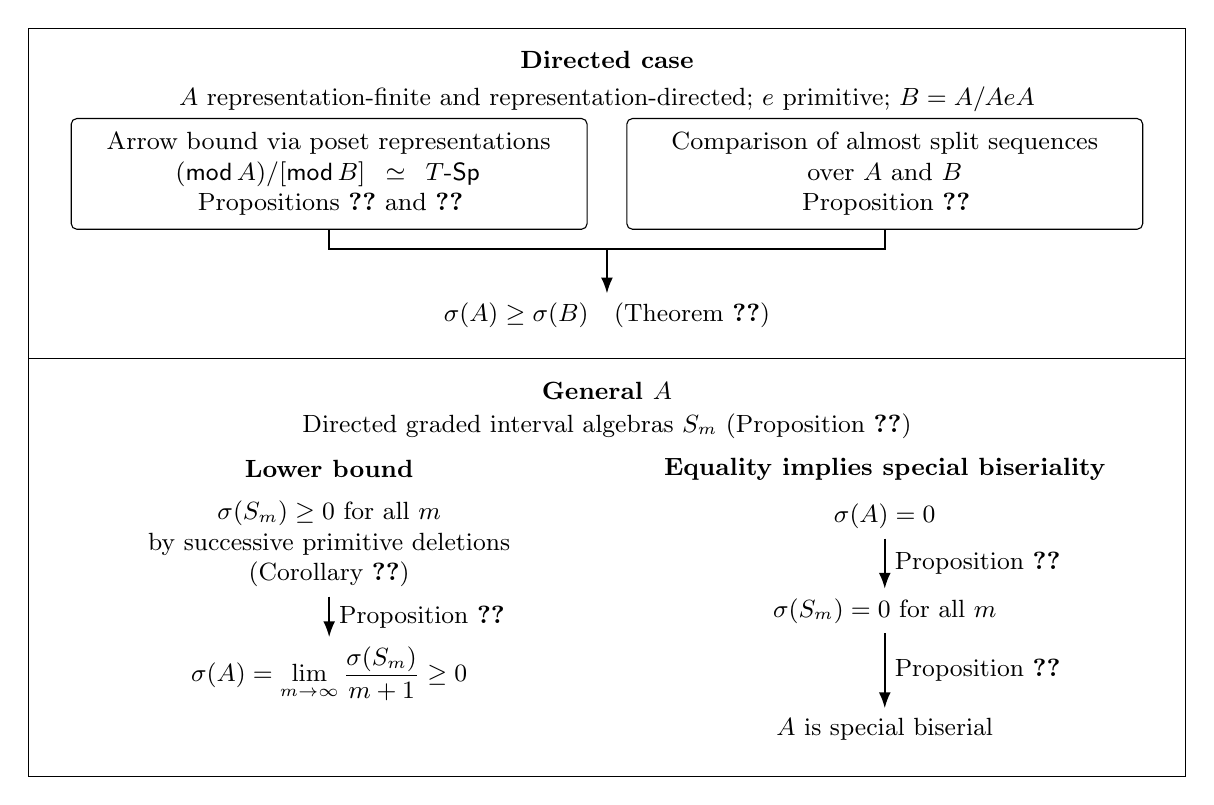
\begin{tikzpicture}[
  x=0.98cm, font=\small,
  every node/.style={align=center},
  input/.style={draw, rounded corners=2pt, text width=6.2cm,
    minimum height=1.25cm, inner sep=5pt},
  implication/.style={-{Latex}, semithick}]
\draw (0,0) rectangle (15,-9.5);
\node[font=\small\bfseries] at (7.5,-0.4) {Directed case};
\node at (7.5,-0.9)
  {\(A\) representation-finite and representation-directed;
   \(e\) primitive; \(B=A/AeA\)};
\node[input] (poset) at (3.9,-1.85)
  {Arrow bound via poset representations\\
   \((\mod A)/[\mod B]\simeq\TSp\)\\
   Propositions~\ref{prop:poset-equivalence} and~\ref{prop:intrinsic}};
\node[input] (sequences) at (11.1,-1.85)
  {Comparison of almost split sequences\\
   over \(A\) and \(B\)\\
   Proposition~\ref{prop:compensation}};
\node (deletion) at (7.5,-3.65)
  {\(\sigma(A)\geq\sigma(B)\)\quad (Theorem~\ref{thm:directed-deletion})};
\draw[semithick] (poset.south) -- (3.9,-2.8) -- (11.1,-2.8)
  -- (sequences.south);
\draw[implication] (7.5,-2.8) -- (deletion.north);
\draw (0,-4.2) -- (15,-4.2);
\node[font=\small\bfseries] at (7.5,-4.6) {General \(A\)};
\node at (7.5,-5.05)
  {Directed graded interval algebras \(S_m\)
   (Proposition~\ref{prop:interval-modules})};
\node[font=\small\bfseries] at (3.9,-5.6) {Lower bound};
\node[font=\small\bfseries] at (11.1,-5.6)
  {Equality implies special biseriality};
\node (nonnegative) at (3.9,-6.55)
  {\(\sigma(S_m)\geq0\) for all \(m\)\\
   by successive primitive deletions\\
   (Corollary~\ref{cor:directed})};
\node (limit) at (3.9,-8.2)
  {\(\displaystyle\sigma(A)=\lim_{m\to\infty}
     \frac{\sigma(S_m)}{m+1}\geq0\)};
\draw[implication] (nonnegative.south) --
  node[right] {Proposition~\ref{prop:interval-count}} (limit.north);
\node (equality) at (11.1,-6.2) {\(\sigma(A)=0\)};
\node (intervals) at (11.1,-7.4)
  {\(\sigma(S_m)=0\) for all \(m\)};
\node (biserial) at (11.1,-8.9) {\(A\) is special biserial};
\draw[implication] (equality.south) --
  node[right] {Proposition~\ref{prop:interval-equality}} (intervals.north);
\draw[implication] (intervals.south) --
  node[right] {Proposition~\ref{prop:equality-forward}} (biserial.north);
\end{tikzpicture}
\caption{Primitive deletion, the lower bound, and the equality case.
 The poset equivalence and arrow bound follow from Ringel--Vossieck \cite{RV}.
 Here \(\sigma(A)=\chi(\mod A)-|A|\), \(\TSp\) denotes
 representations of a finite poset \(T\) by subspaces, \(S\) is a
 standard form of \(A\), and \(\mod S_m\) is equivalent to the category
 of graded \(S\)-modules supported in degrees \(0,\ldots,m\)
 (Proposition~\ref{prop:interval-modules}).}
\label{fig:proof-overview}
\end{figure}

\begin{organization}
Section~\ref{sec:ar} recalls the magnitude formula, almost split sequences,
and their generalization to \(\tau\)-categories.
For a directed algebra, Section~\ref{sec:quotient} describes the additive
quotient and its \(\tau\)-sequences using Iyama's quotient theorem
(Proposition~\ref{prop:quotient-sequences}). It gives the poset representation
equivalence and deduces an arrow bound from Ringel--Vossieck's results.
Section~\ref{sec:deletion} combines this bound with a comparison of almost
split sequences to prove Theorem~\ref{thm:directed-deletion}.
Section~\ref{sec:general} constructs finite algebras from graded modules
over the standard form and applies the directed result to prove both
assertions of Theorem~A. Appendix~\ref{app:structural} proves the structural
results on the quotient directly and gives the detailed example for the
Dynkin quiver of type \(D_4\) (Example~\ref{ex:d4-details}).
\end{organization}

\begin{conventions}
Throughout, \(k\) is algebraically closed and algebras are finite-dimensional
\(k\)-algebras. Modules are finite-dimensional right modules, and
\(\mod A\) denotes their category. We write \(\Dk=\Hom_k(-,k)\), and
\(\add M\) for direct summands of finite direct sums of copies of \(M\).
For a Krull--Schmidt category \(\cC\), \(\ind\cC\) is a chosen set
of indecomposable representatives, also regarded as the full subcategory
on those objects. We write \(\cC(X,Y)=\Hom_{\cC}(X,Y)\) and abbreviate
\(\ind(\mod A)\) to \(\ind A\). A category is representation-finite
if it has finitely many indecomposable isomorphism classes.
The categorical radical is \(\rad_{\cC}\), and
\(\Irr_{\cC}(X,Y)=\rad_{\cC}(X,Y)/\rad_{\cC}^2(X,Y)\).
The \emph{irreducible quiver} of \(\cC\) has vertices \(\ind\cC\)
and \(\dim_k\Irr_{\cC}(X,Y)\) arrows from \(X\) to \(Y\).
We write \(\indeg_{\cC}(X)\) and \(\outdeg_{\cC}(X)\) for the
numbers of incoming and outgoing arrows, including multiplicities.
The \emph{Auslander--Reiten translation quiver} \(\Gamma_A\) is this
quiver of \(\mod A\), equipped with Auslander--Reiten translation and
with its projective and injective vertices marked.
Translations are displayed by dotted arrows
\(X\dashrightarrow\tau_A X\); they do not count as arrows in paths
or arrow counts.
An algebra is \emph{representation-directed} if there is no cycle of
nonzero nonisomorphisms between indecomposable modules. We also use
\emph{directed} in this sense for a category. Composition is written
\(gf\) for first \(f\), then \(g\). We use the same order for paths:
\(\beta\alpha\) traverses \(\alpha\) first, then \(\beta\).
\end{conventions}

\begin{aiuse}
The research was conducted under the author's direction using GPT-5.6-Sol,
Claude Fable~5, Claude Opus~5, and GPT-6-Astra. GPT-5.6-Sol and Claude Fable~5 developed
the initial proof, and GPT-5.6-Sol produced earlier manuscript drafts.
GPT-6-Astra subsequently developed the simplified proof presented here and
wrote a new manuscript based on it, retaining selected arguments and examples
from the earlier drafts. Claude Opus~5 extensively reviewed the proofs and
successive manuscript drafts. The author directed the research and revisions and
set the structure and much of the wording of the present text. The author
is responsible for the mathematical content and the final manuscript.
\end{aiuse}

\section{Magnitude and almost split sequences}\label{sec:ar}
The magnitude formula expresses the problem in terms of the numbers of
indecomposable modules, simple modules, and arrows in the Auslander--Reiten quiver.
We recall this formula
and the properties of almost split sequences used in the quotient argument.

\subsection{The counting formula}
Fix a representation-finite algebra \(A\).

\begin{definition}\label{def:surplus}
Put
\[
 a(A)=\sum_{X,Y\in\ind A}\dim_k\Irr_A(X,Y),\qquad
 \sigma(A)=\chi(\mod A)-|A|.
\]
We call \(\sigma(A)\) the \emph{magnitude surplus}.
\end{definition}

The following formula expresses magnitude in terms of these counts.
\begin{lemma}[{\cite[Lemma~1.9]{BHK}}]\label{lem:count}
The matrix \(H_A=(\dim_k\Hom_A(X,Y))_{X,Y\in\ind A}\) is invertible, and
\[
 \chi(\mod A)=2|\ind A|-|A|-a(A).
\]
Consequently,
\begin{equation}\label{eq:count}
 \sigma(A)=2(|\ind A|-|A|)-a(A).
\end{equation}
\end{lemma}

We use Morita equivalence to reduce to basic algebras and additivity to
count the surplus of products of interval algebras in Section~\ref{sec:general}.
\begin{lemma}\label{lem:invariance}
Magnitude, \(|A|\), and \(\sigma(A)\) are Morita invariant and additive
on products of algebras.
\end{lemma}
\begin{proof}
A \(k\)-linear Morita equivalence preserves simple classes, indecomposable
classes, and Hom dimensions. For a product of algebras, the Hom matrix is
block diagonal, so its inverse is block diagonal and its entry sum is the
sum for the factors. The simple classes are the disjoint union of those of
the factors. Subtracting their numbers proves the assertion for \(\sigma\).
\end{proof}

\begin{remark}\label{rem:deletion-morita}
We call passage from \(A\) to \(A/AeA\), for a primitive idempotent
\(e\), \emph{primitive deletion}. To study it over a basic algebra,
choose an idempotent \(f\) with \(fe=ef=e\), \(AfA=A\), and
\(fAf\) basic. From a complete orthogonal set of primitive idempotents
containing \(e\), take one for each isomorphism class of indecomposable
projectives, including \(e\), and let \(f\) be their sum.
The idempotent \(e\) remains primitive in \(fAf\), since
\(e(fAf)e=eAe\) is local.
Since \((Xf)e=Xe\), the Morita equivalence \(X\mapsto Xf\) restricts to
\[
 \mod(A/AeA)\simeq\mod\bigl(fAf/(fAf)e(fAf)\bigr).
\]
Indeed, \(f(AeA)f=(fAf)e(fAf)\). Writing \(\bar f\) for the image of
\(f\) in \(B=A/AeA\), the equality \(AfA=A\) gives \(B\bar fB=B\),
so \(\bar f\) is full and induces the displayed Morita equivalence.
By Lemma~\ref{lem:invariance}, this reduction preserves
\(\sigma(A)-\sigma(A/AeA)\).
\end{remark}

\subsection{Almost split maps and \texorpdfstring{\(\tau\)}{tau}-sequences}
We recall almost split maps and sequences, then define the
\(\tau\)-sequences used in the additive quotient.

A map \(f:V\to X\) to an indecomposable \(X\) is \emph{right almost split}
if it is not a retraction and every non-retraction to \(X\) factors through it.
It is \emph{right minimal} if every \(u\in\End(V)\) with \(fu=f\)
is invertible. Left almost split maps and left minimality are defined dually,
using sections.

\begin{definition}\label{def:ar}
For a nonprojective indecomposable \(X\), write its almost split sequence as
\[
 0\longrightarrow\tau_A X\longrightarrow\theta_A X
 \longrightarrow X\longrightarrow0.
\]
At a projective \(X\), put \(\tau_A X=0\), \(\theta_A X=\rad X\), and
use the radical inclusion \(\theta_A X\to X\).
Dually, write the sequence starting at a noninjective \(X\) as
\[
 0\longrightarrow X\longrightarrow\theta_A^-X
 \longrightarrow\tau_A^-X\longrightarrow0,
\]
and put \(\theta_A^-X=X/\soc X\), \(\tau_A^-X=0\) at an injective \(X\).
Extend \(\tau_A,\tau_A^-,\theta_A,\theta_A^-\) additively to arbitrary
modules, as assignments on isomorphism classes.
\end{definition}

The following standard facts relate almost split maps to the arrows of
\(\Gamma_A\). For an indecomposable \(Y\), write \([V:Y]_\oplus\)
for its multiplicity as a direct summand of \(V\).

\begin{proposition}[{\cite[V, Section~1; VII, Proposition~1.3]{ARS}}]\label{prop:ar-multiplicity}
For indecomposable \(A\)-modules \(X,Y\), the maps
\(\theta_A X\to X\) are minimal right almost split and the maps
\(X\to\theta_A^-X\) are minimal left almost split. Their middle
multiplicities satisfy
\begin{equation}\label{eq:ar-multiplicity}
 [\theta_A X:Y]_\oplus=\dim_k\Irr_A(Y,X),\qquad
 [\theta_A^-X:Y]_\oplus=\dim_k\Irr_A(X,Y).
\end{equation}
The map \(\tau_A\) is a bijection from nonprojective to noninjective
indecomposables, with inverse \(\tau_A^-\).
\end{proposition}

We will use the following form of Auslander--Reiten duality.
\begin{proposition}[{\cite[IV, Theorem~2.13]{ASS}}]\label{prop:ar-duality}
For modules \(U,V\), there are natural isomorphisms
\begin{equation}\label{eq:ar-duality}
 \Dk\Ext_A^1(U,V)\cong\uhom_A(\tau_A^-V,U)
 \cong\ohom_A(V,\tau_A U).
\end{equation}
Here \(\uhom\) is Hom modulo maps through projectives, and \(\ohom\)
is Hom modulo maps through injectives. The formulas include the zero cases
when \(V\) is injective or \(U\) is projective.
\end{proposition}

An additive quotient need not be an abelian category. To describe the
images of almost split sequences in such a quotient, we use weak kernels
and weak cokernels, which we now recall.
\begin{definition}\label{def:weak-kernel}
In an additive category, a map \(f:L\to V\) is a \emph{weak kernel} of
\(g:V\to Y\) if \(gf=0\) and every map \(h:Z\to V\) with \(gh=0\)
factors through \(f\). It is minimal if \(fu=f\) forces \(u\in\End(L)\)
to be invertible. Weak cokernels and their minimality are defined dually.
\end{definition}

\begin{definition}[{\cite[Section~1.3]{IyamaIV}}]\label{def:tau-category}
Let \(\cC\) be a Krull--Schmidt category. A complex
\(L\xrightarrow{f}V\xrightarrow{g}Y\) is a \emph{right \(\tau\)-sequence}
if \(f,g\) are radical, \(f\) is a minimal weak kernel of \(g\), and
for every object \(Z\),
\[
 \operatorname{Im}\bigl(\cC(V,Z)\xrightarrow{-\circ f}\cC(L,Z)\bigr)
       =\rad_{\cC}(L,Z),\qquad
 \operatorname{Im}\bigl(\cC(Z,V)\xrightarrow{g\circ-}\cC(Z,Y)\bigr)
       =\rad_{\cC}(Z,Y).
\]
A \emph{left \(\tau\)-sequence} satisfies the same radical and image
conditions, with \(g\) a minimal weak cokernel of \(f\).
The category \(\cC\) is a \emph{\(\tau\)-category} if every indecomposable
is the last term of a right \(\tau\)-sequence and the first term of a
left \(\tau\)-sequence.
\end{definition}
Since \(f,g\) are radical, their composites with arbitrary maps are radical.
The two image equalities therefore say that every radical map out of \(L\)
factors through \(f\), and every radical map into \(Y\) factors through \(g\).
\begin{remark}[{\cite[Sections~2.1 and~2.3]{IyamaI}}]\label{rem:tau-properties}
At an indecomposable last term, the last map
of a right \(\tau\)-sequence is minimal right almost split, and the first
term is either zero or indecomposable. Dually, the first map of a left
\(\tau\)-sequence starting at an indecomposable is minimal left almost split,
and its last term is either zero or indecomposable. A right \(\tau\)-sequence
is determined up to isomorphism by its indecomposable last term, and a left
\(\tau\)-sequence by its indecomposable first term.
A right \(\tau\)-sequence with nonzero indecomposable endpoints
is also a left \(\tau\)-sequence, and conversely. Thus taking the first term
of a right \(\tau\)-sequence gives a bijection from the indecomposables
whose right \(\tau\)-sequence has nonzero first term to those whose
left \(\tau\)-sequence has nonzero last term;
its inverse takes the last term of the left \(\tau\)-sequence.
\end{remark}
\begin{example}\label{ex:module-tau}
The category \(\mod A\) is a \(\tau\)-category: its right and left
\(\tau\)-sequences are the
almost split sequences with their outer zeros omitted, together with
\(0\to\rad P\to P\) at projectives and
\(I\to I/\soc I\to0\) at injectives.
The almost split factorization properties give the two image equalities
in Definition~\ref{def:tau-category}; the ordinary kernels and cokernels
give the required minimal weak kernels and cokernels.
\end{example}

We will repeatedly express radical maps as sums of composites of irreducible maps.
\begin{lemma}\label{lem:path-expansion}
Let \(\cC\) be a Hom-finite Krull--Schmidt \(k\)-category with finitely
many indecomposable isomorphism classes. Choose maps representing a basis
of each \(\Irr_{\cC}(X,Y)\). Then its radical is nilpotent, and every
radical map between indecomposables is a linear combination of nonempty
paths in the chosen maps.
\end{lemma}
\begin{proof}
Put \(M=\bigoplus_{X\in\ind\cC}X\) and \(\Lambda=\End_{\cC}(M)\).
The spaces \(\rad_{\cC}(X,Y)\) are the corresponding matrix blocks of
\(\rad\Lambda\). Since \(\Lambda\) is finite-dimensional, choose \(N\)
with \((\rad\Lambda)^N=0\); then \(\rad_{\cC}^N=0\).
Modulo \(\rad_{\cC}^2\), every radical map
is a linear combination of the chosen representatives. Repeating this
expansion in each factor expresses it modulo \(\rad_{\cC}^{n+1}\)
as a sum of paths of lengths at most \(n\). Taking \(n=N-1\) proves the claim.
\end{proof}
\section{The quotient and its poset representations}\label{sec:quotient}
For a directed algebra and a primitive idempotent \(e\), we form an
additive quotient whose indecomposable objects are the indecomposable
\(A\)-modules \(X\) with \(Xe\ne0\).
Iyama's quotient theorem describes its \(\tau\)-sequences, and
Ringel--Vossieck's results identify it with a category of poset representations.
We state these results in terms of the quotient and use them to bound the
number of its irreducible arrows. This bound will give one of the
nonnegative contributions to the change in magnitude under deletion.
The proofs of the multiplicity, height, and poset results are given in
Appendix~\ref{app:structural}.

\begin{setting}\label{set:directed}
Throughout Sections~\ref{sec:quotient}--\ref{sec:deletion} and Appendix~\ref{app:structural}, let \(A\) be
basic, representation-finite, and representation-directed. Fix a primitive
idempotent \(e\), and put
\[
 J=AeA,\quad B=A/J,\quad \cD=(\mod A)/[\mod B],\quad
 P=eA,\quad E=P/\rad P,\quad I=\Dk(Ae).
\]
Thus \(P\) is the projective cover of the simple module \(E\), and
\(I\) is its injective envelope.
The quotient has the same objects as \(\mod A\); its morphisms are taken
modulo maps factoring through \(B\)-modules. We regard \(\mod B\) as the
full subcategory of modules \(X\) with \(Xe=0\), by restriction of scalars
along \(A\twoheadrightarrow B\). Put
\(d_X=\dim_k Xe=[X:E]\), where \([X:E]\) is composition multiplicity.
The equality follows by applying the exact functor \((-)e\) to a
composition series.
\end{setting}

\begin{lemma}\label{lem:quotient-closure}
The subcategory \(\mod B\) of \(\mod A\) is closed under submodules,
quotients, extensions and direct summands. The algebra \(B\) is
representation-finite and representation-directed.
For every \(W\in\mod B\),
\(\Hom_A(E,W)=\Hom_A(W,E)=0\).
\end{lemma}
\begin{proof}
Submodules and quotients of modules annihilated by \(J\) are again
annihilated by \(J\). For extension closure, let \(0\to X\to V\to Y\to0\)
be exact with \(XJ=YJ=0\). Then \(VJ\subseteq X\). Since \(e^2=e\),
the ideal \(J=AeA\) satisfies \(J^2=J\), so
\(VJ=VJ^2\subseteq XJ=0\).
Moreover, \(\mod B\) is a full subcategory of \(\mod A\) closed under
direct summands. The inclusion preserves indecomposables and their Hom
spaces, so \(B\) is representation-finite and directed.
Finally, \(We=0\) implies \([W:E]=0\), so \(E\) is neither a
submodule nor a quotient of \(W\). This proves both Hom vanishings.
\end{proof}

\subsection{Evaluation and irreducible maps in the quotient}
We first show that the indecomposable objects of \(\cD\) are precisely
the indecomposable \(A\)-modules \(X\) with \(Xe\ne0\). We also show
that a map becomes zero in \(\cD\) if and only if its restriction at
\(e\) is zero. For a module map
\(f:X\to Y\), write \(f_e:Xe\to Ye\) for its restriction.

\begin{lemma}\label{lem:evaluation}
Evaluation at \(e\) and passage to \(\cD\) have the following properties.
\begin{enumerate}
\item The functor \(F:\cD\to\mod k\), sending \(X\) to \(Xe\) and
 the class of \(f\) to \(f_e\), is faithful.
\item Every indecomposable \(A\)-module has endomorphism ring \(k\).
The category \(\cD\) is Krull--Schmidt and directed. Its indecomposables
 are the images of the indecomposable \(A\)-modules with \(d_X>0\);
 they remain distinct and have endomorphism ring \(k\).
\item For every object \(X\),
\begin{equation}\label{eq:evaluation}
 \cD(P,X)=\Hom_A(P,X)\cong Xe,\qquad
 \cD(X,I)=\Hom_A(X,I)\cong\Dk(Xe).
\end{equation}
The object \(P\) is the unique source and \(I\) the unique sink of the
irreducible quiver of \(\cD\).
\end{enumerate}
\end{lemma}
\begin{proof}
(1) If \(f_e=0\), then \(f\) kills \(XeA\) and factors through the
\(B\)-module \(X/XeA\). Conversely, a factorization through a
\(B\)-module has zero evaluation. This proves faithfulness.

(2) Directedness gives \(\End_A(X)=k\) for every indecomposable \(X\): a
nonzero noninvertible endomorphism would be a cycle, and a finite-dimensional
division algebra over the algebraically closed field \(k\) is \(k\).
For \(d_X>0\), the ideal of maps through \(B\) is zero in this ring,
since a factorization of \(1_X\) through a \(B\)-module would make \(X\)
a direct summand of that module and force \(Xe=0\).
Hence \(X\) remains indecomposable.
If \(f:X\to Y\) and \(g:Y\to X\) lift inverse isomorphisms in the
quotient, then \(gf-1_X\) and \(fg-1_Y\) belong to these zero ideals.
Thus \(f,g\) are inverse over \(A\), and nonisomorphic indecomposable
\(A\)-modules with nonzero evaluation at \(e\) remain nonisomorphic in \(\cD\). Lifting a cycle of nonzero nonisomorphisms would
give one over \(A\), so the quotient is directed.

Every object of \(\cD\) is a finite sum of indecomposables with endomorphism ring \(k\),
so \(\cD\) is Krull--Schmidt.

(3) The identifications in \eqref{eq:evaluation} hold because
\(\Hom_A(P,\mod B)=0\) and \(\Hom_A(\mod B,I)=0\).
Every indecomposable of \(\cD\) therefore receives a nonzero map from \(P\) and maps
nontrivially to \(I\). An incoming arrow at \(P\), or an outgoing arrow
at \(I\), would give a cycle. Expanding the nonzero maps from \(P\) and to \(I\)
into paths by Lemma~\ref{lem:path-expansion} gives an incoming arrow at
every \(X\ne P\) and an outgoing arrow at every \(X\ne I\), by taking
the last and first arrows of these paths, respectively.
\end{proof}

We next identify the arrows that contribute to the quotient's arrow count.
\begin{lemma}\label{lem:surviving-arrows}
Let \(X,Y\) be indecomposable \(A\)-modules with \(Xe\ne0\) and
\(Ye\ne0\). The quotient functor induces an isomorphism
\[
 \Irr_A(X,Y)\cong\Irr_{\cD}(X,Y).
\]
\end{lemma}
\begin{proof}
Both factors of a map through an indecomposable \(B\)-module are radical,
so \([\mod B](X,Y)\subseteq\rad_A^2(X,Y)\). If \(X\not\cong Y\),
their images remain nonisomorphic by Lemma~\ref{lem:evaluation}(2),
so every map between them is radical in both categories.
If \(X\cong Y\), both radical spaces are zero, since
\(\End_A(X)=\End_{\cD}(X)=k\).
Thus the quotient map sends \(\rad_A(X,Y)\) onto
\(\rad_{\cD}(X,Y)\), with kernel \([\mod B](X,Y)\subseteq\rad_A^2(X,Y)\).
A composite of radical maps through an indecomposable with nonzero evaluation
at \(e\) lifts to such a composite over \(A\); a composite through a \(B\)-module becomes zero.
The image of \(\rad_A^2(X,Y)\) is therefore \(\rad_{\cD}^2(X,Y)\),
so the induced map on radical quotients is both surjective and injective.
\end{proof}

\subsection{The inherited \texorpdfstring{\(\tau\)}{tau}-sequences}
By Lemma~\ref{lem:surviving-arrows}, the quotient preserves irreducible
maps between indecomposables with nonzero evaluation at \(e\). Their
Auslander--Reiten translates over \(A\), however, may belong to \(\mod B\)
and hence become zero in \(\cD\). The following proposition describes
the resulting \(\tau\)-category structure; bars denote images under
\(\mod A\to\cD\).

\begin{proposition}[{\cite[Section~1.4(2),(3)]{IyamaII}}]\label{prop:quotient-sequences}
The category \(\cD\) is a \(\tau\)-category. For an indecomposable
\(A\)-module \(X\) with \(Xe\ne0\), its right and left \(\tau\)-sequences are
\[
 \overline{\tau_A X}\longrightarrow\overline{\theta_A X}
       \longrightarrow X,
 \qquad
 X\longrightarrow\overline{\theta_A^-X}
       \longrightarrow\overline{\tau_A^-X},
\]
using the projective and injective conventions of Definition~\ref{def:ar}.
Thus each term is obtained by deleting its indecomposable summands in
\(\mod B\).
\end{proposition}

\begin{proof}
Iyama's result \cite[Section~1.4(2),(3)]{IyamaII} states that the quotient
of a \(\tau\)-category by a full additive subcategory closed under direct
summands is again a \(\tau\)-category. At a surviving indecomposable,
the right \(\tau\)-sequence is the image of the original one when the
image of its middle term is nonzero; otherwise it is \(0\to0\to X\).
The dual statement gives the left \(\tau\)-sequences.
Example~\ref{ex:module-tau} applies to \(\mod A\), and \(\mod B\)
is a full additive subcategory closed under direct summands.
It remains to check that the displayed images also have the stated form
when a middle term vanishes. Indeed,
if \(X\) is nonprojective over \(A\), applying \((-)e\) to its almost split
sequence over \(A\) gives
\(d_{\theta_A X}=d_{\tau_A X}+d_X>0\). Its middle term is therefore
nonzero in the quotient. If the middle term becomes zero, \(X\) must
therefore be projective over \(A\). Then \(\tau_A X=0\), and the
displayed image sequence is exactly \(0\to0\to X\), as required.
The same argument applies to left \(\tau\)-sequences by duality.
\end{proof}
We now fix notation for the inherited terms and the objects with zero translate.

\begin{definition}\label{def:boundary}
For \(X\in\ind\cD\), write the inherited sequences as
\[
 \tau^+X\longrightarrow\theta^+X\longrightarrow X,
 \qquad X\longrightarrow\theta^-X\longrightarrow\tau^-X.
\]
Here
\(\tau^+X\) is the image of \(\tau_A X\), and similarly on the left;
the sequences at projective and injective \(A\)-modules are included.
Following the notation of \cite[Section~2.1(3)]{IyamaI}, put
\[
 \ind_1^+\cD=\{X:\tau^+X=0\},\qquad
 \ind_1^-\cD=\{X:\tau^-X=0\}.
\]
Their members are called \emph{\(\tau\)-projective} and
\emph{\(\tau\)-injective}, respectively. Their union is the boundary.
Write \(\Gamma_{\cD}\) for the irreducible quiver of \(\cD\) equipped
with this translation, displayed by dotted arrows \(X\dashrightarrow\tau^+X\).
\end{definition}

\begin{remark}\label{rem:iyama-boundary}
Let \(X\) be an indecomposable \(A\)-module with \(Xe\ne0\).
Its image is \(\tau\)-projective in \(\cD\) precisely when \(X\) is
projective over \(A\) or \(\tau_A X\) belongs to \(\mod B\).
In particular, an object can be \(\tau\)-projective in \(\cD\) without
being projective over \(A\). The dual statement holds for
\(\tau\)-injectives.
\end{remark}

The inherited sequences give the following identities, which we will use
in the arrow count and the multiplicity bounds.

\begin{lemma}\label{lem:quotient-identities}
In Setting~\ref{set:directed}, the following hold.
\begin{enumerate}
\item The boundary sets have the same cardinality:
\begin{equation}\label{eq:boundary-cardinality}
 |\ind_1^+\cD|=|\ind_1^-\cD|.
\end{equation}
\item For \(X,Y\in\ind\cD\), the middle multiplicities are
\begin{equation}\label{eq:quotient-multiplicity}
 [\theta^+X:Y]_\oplus=\dim_k\Irr_{\cD}(Y,X),\qquad
 [\theta^-X:Y]_\oplus=\dim_k\Irr_{\cD}(X,Y).
\end{equation}
\item If \(\tau^+X\ne0\), then for every \(Y\in\ind\cD\),
\begin{equation}\label{eq:paired-middle}
 \theta^-(\tau^+X)\cong\theta^+X,
 \qquad\dim_k\Irr_{\cD}(Y,X)=\dim_k\Irr_{\cD}(\tau^+X,Y).
\end{equation}
\item For \(X\in\ind\cD\), evaluation at \(e\) satisfies
\begin{equation}\label{eq:dimension-defects}
 d_X-d_{\theta^+X}+d_{\tau^+X}=\indicator_{\{X=P\}},\qquad
 d_X-d_{\theta^-X}+d_{\tau^-X}=\indicator_{\{X=I\}}.
\end{equation}
Here \(\indicator_{\{X=P\}}\) is one if \(X\cong P\) and zero
otherwise, and similarly for \(I\).
\end{enumerate}
\end{lemma}
\begin{proof}
(1) Remark~\ref{rem:tau-properties} gives inverse bijections
\[
 \tau^+:\ind\cD\setminus\ind_1^+\cD
 \longleftrightarrow\ind\cD\setminus\ind_1^-\cD:\tau^-.
\]
Since \(\ind\cD\) is finite, their complements have equal cardinality.

(2) Proposition~\ref{prop:quotient-sequences} deletes only the
\(B\)-summands from the middle terms. Lemma~\ref{lem:surviving-arrows}
identifies the remaining irreducible spaces with those in
\eqref{eq:ar-multiplicity}, proving \eqref{eq:quotient-multiplicity}.

(3) By Remark~\ref{rem:tau-properties}, the right \(\tau\)-sequence at
\(X\) is also the left \(\tau\)-sequence at \(\tau^+X\). Their
middle terms agree, and (2) gives the equality of arrow multiplicities.

(4) Deleted \(B\)-summands have zero evaluation at \(e\), so they do not
change \(d\) for any term. For a nonprojective \(A\)-module, the first
identity follows by applying the exact functor \((-)e\) to its almost
split sequence. At a projective it is
\(d_X-d_{\rad X}=[\operatorname{top}X:E]\). An indecomposable
projective has simple top, so this multiplicity is one precisely when
\(X\cong P\), and zero otherwise. The second identity is dual.
\end{proof}

\subsection{Multiplicity one}
The multiplicity bounds below are consequences of Ringel--Vossieck's results
on finite hammocks. In their application to directed algebras, these include
the estimate of V.~H\"ohne recorded in \cite[Section~10, p.~243]{RV}.
Besides determining the arrows at the boundary of \(\cD\), the bounds
control the endpoints of the almost split sequences compared in
Section~\ref{sec:deletion}.

\begin{proposition}[{\cite[Section~1, Corollary~3; Section~10, p.~243]{RV}}]\label{prop:boundary-one}
In Setting~\ref{set:directed}, the following hold.
\begin{enumerate}
\item Every \(\tau\)-projective and \(\tau\)-injective of \(\cD\) has
\(d_X=1\).
\item Every indecomposable projective or injective \(A\)-module has \(d_X\leq1\).
\item For an almost split sequence \(0\to X\to V\to Y\to0\) over \(A\),
\begin{equation}\label{eq:zero-end}
 Xe=0\ \Longrightarrow\ d_Y\leq1,\qquad
 Ye=0\ \Longrightarrow\ d_X\leq1.
\end{equation}
\end{enumerate}
\end{proposition}
A direct proof is given in Appendix~\ref{app:multiplicity}.

\begin{corollary}\label{cor:boundary-arrows}
In \(\Gamma_{\cD}\), each \(\tau\)-projective other than \(P\) has exactly one incoming
arrow, with multiplicity one; \(P\) has none. Dually, each
\(\tau\)-injective other than \(I\) has exactly one outgoing arrow,
and \(I\) has none.
\end{corollary}
\begin{proof}
For a \(\tau\)-projective \(X\ne P\), equation
\eqref{eq:dimension-defects} gives \(d_{\theta^+X}=d_X=1\).
Every indecomposable summand of \(\theta^+X\) has positive integral
dimension at \(e\), so there is exactly one, occurring once. Equation~\eqref{eq:quotient-multiplicity}
then gives the incoming arrow count. For \(P\), Lemma~\ref{lem:evaluation}(2),(3)
gives \(d_P=\dim_k\End_A(P)=1\), so equation
\eqref{eq:dimension-defects} gives \(d_{\theta^+P}=0\). Thus there are no
incoming arrows. The second formula in \eqref{eq:dimension-defects}
gives the outgoing counts by the same argument.
\end{proof}

The following example shows how deleting modules changes the translation
and produces additional \(\tau\)-projective objects.
\begin{example}\label{ex:a3}
Let \(Q\) be \(1\to2\to3\) and \(A=(kQ)^\op\). Thus right
\(A\)-modules are representations in the displayed direction. Write
\(M_{ij}\) for the interval representation on vertices \(i,\ldots,j\),
with identity maps between nonzero coordinates, and \(S_i=M_{ii}\).
The Auslander--Reiten translation quiver of \(A\) is
\[
\begin{tikzcd}
 &&M_{13}\arrow[dr]&&\\
 &M_{23}\arrow[ur]\arrow[dr]&&M_{12}\arrow[dr]
   \arrow[ll,dotted,"\tau_A"']&\\
 S_3\arrow[ur]&&S_2\arrow[ur]\arrow[ll,dotted,"\tau_A"']&&
 S_1\arrow[ll,dotted,"\tau_A"']
\end{tikzcd}
\]
Take \(e\) to be the vertex idempotent at \(2\), so \(E=S_2\).
Then \(B\cong k\times k\), whose indecomposables
\(S_1,S_3\) become zero in \(\cD\). The quotient has translation quiver
\[
\begin{tikzcd}
 &M_{13}\arrow[dr]&\\
 P=M_{23}\arrow[ur]\arrow[dr]&&M_{12}=I\arrow[ll,dotted,"\tau^+"']\\
 &S_2\arrow[ur]&
\end{tikzcd}
\]
The only nonzero translate is \(\tau^+M_{12}=M_{23}\). In particular,
the right \(\tau\)-sequence at \(S_2\) has first term zero because its
first term over \(A\) is \(S_3\). Hence
\(\ind_1^+\cD=\{M_{23},M_{13},S_2\}\). Each has dimension one at
vertex 2, as does \(I=M_{12}\).
\end{example}
\subsection{Path lengths and the number of arrows}\label{subsec:heights}
The boundary arrows determine the lengths of paths in \(\Gamma_{\cD}\).
We use these lengths to prove the bound
\(a(\cD)\leq2|\ind\cD|-|\ind_1^+\cD|-1\) needed for deletion.

\begin{definition}\label{def:epsilon}
Let \(a(\cD)=\sum_{X,Y\in\ind\cD}\dim_k\Irr_{\cD}(X,Y)\), and put
\[
 \eps(\cD)=2|\ind\cD|-a(\cD)-|\ind_1^+\cD|-1.
\]
Thus the desired arrow bound is equivalent to \(\eps(\cD)\geq0\).
\end{definition}

The quiver \(\Gamma_{\cD}\) is finite with unique source \(P\), and each
\(\tau\)-projective has at most one incoming arrow, by
Lemma~\ref{lem:evaluation}(3) and Corollary~\ref{cor:boundary-arrows}.
The lemma of Ringel--Vossieck \cite[Section~7, pp.~234--235]{RV} gives
the grading property: all paths of irreducible maps from \(P\) to a fixed
indecomposable have the same length. Together with
Lemma~\ref{lem:path-expansion}, this gives the height function and radical
identities below.

\begin{proposition}\label{prop:height}
There is a unique function \(h:\ind\cD\to\mathbb Z_{\geq0}\), called
the \emph{height}, with \(h(P)=0\)
such that every arrow \(X\to Y\) satisfies \(h(Y)=h(X)+1\), and
\(h(X)=h(\tau^+X)+2\) whenever \(\tau^+X\ne0\).
For distinct \(X,Y\) with \(\cD(X,Y)\ne0\), put \(\ell=h(Y)-h(X)\).
Then \(\ell>0\) and
\begin{equation}\label{eq:height-radical}
 \cD(X,Y)=\rad_{\cD}^{\ell}(X,Y),\qquad
 \rad_{\cD}^{\ell+1}(X,Y)=0.
\end{equation}
Put \(L=h(I)\). All heights lie in \([0,L]\), with \(P,I\) the unique
objects of heights \(0,L\), respectively.
\end{proposition}
A direct proof is given in Appendix~\ref{app:heights}.

The next count reduces the arrow bound to
\(L\geq|\ind_1^+\cD|-1\), where \(L=h(I)\).
\begin{lemma}\label{lem:height-count}
With \(L=h(I)\), one has
\begin{equation}\label{eq:height-count}
 a(\cD)=2|\ind\cD|-L-2,\qquad
 \eps(\cD)=L-(|\ind_1^+\cD|-1).
\end{equation}
\end{lemma}
\begin{proof}
Put \(H_+=\sum_{X\in\ind_1^+\cD}h(X)\) and
\(H_-=\sum_{X\in\ind_1^-\cD}h(X)\).
The map \(\tau^+\) gives a bijection from the non-\(\tau\)-projectives to the
non-\(\tau\)-injectives. Hence
\[
\begin{aligned}
 \sum_{X\notin\ind_1^+\cD}h(X)
 &=\sum_{X\in\ind\cD}h(X)-H_+,\\
 \sum_{X\notin\ind_1^+\cD}h(\tau^+X)
 &=\sum_{Y\notin\ind_1^-\cD}h(Y)
 =\sum_{Y\in\ind\cD}h(Y)-H_-.
\end{aligned}
\]
Summing \(h(X)-h(\tau^+X)=2\) over the non-\(\tau\)-projectives gives
\[
 H_--H_+=2(|\ind\cD|-|\ind_1^+\cD|).
\]
Every arrow contributes the height of its target minus that of its source,
which is one. Thus
\[
 a(\cD)=\sum_Xh(X)\indeg_{\cD}(X)-\sum_Xh(X)\outdeg_{\cD}(X).
\]
For a non-\(\tau\)-projective \(X\), equation~\eqref{eq:paired-middle}
gives \(\indeg_{\cD}(X)=\outdeg_{\cD}(\tau^+X)\). Reindexing by
\(Y=\tau^+X\) and using Corollary~\ref{cor:boundary-arrows} gives
\[
 \sum_Xh(X)\indeg_{\cD}(X)
 =\sum_{Y\notin\ind_1^-\cD}(h(Y)+2)\outdeg_{\cD}(Y)+H_+.
\]
Here the boundary contribution is \(H_+\), since every \(\tau\)-projective
except \(P\) has indegree one and \(h(P)=0\). Similarly, every
\(\tau\)-injective except \(I\) has outdegree one, so
\[
 \sum_{Y\in\ind_1^-\cD}h(Y)\outdeg_{\cD}(Y)=H_--L,\qquad
 \sum_{Y\in\ind_1^-\cD}\outdeg_{\cD}(Y)=|\ind_1^-\cD|-1.
\]
Subtracting the outgoing weighted sum, we obtain
\[
 \begin{aligned}
 a(\cD)
 &=2\sum_{Y\notin\ind_1^-\cD}\outdeg_{\cD}(Y)+H_+-H_-+L\\
 &=2\bigl(a(\cD)-|\ind_1^+\cD|+1\bigr)
   -2\bigl(|\ind\cD|-|\ind_1^+\cD|\bigr)+L.
 \end{aligned}
\]
In the second equality, we subtract the boundary outdegree from the total
outdegree \(a(\cD)\), then use \eqref{eq:boundary-cardinality} and the
formula for \(H_--H_+\).
Solving gives the first formula; substitution in
Definition~\ref{def:epsilon} gives the second. The same calculation includes
\(P=I\), when there is one object and no arrows.
\end{proof}

\subsection{The poset and its representations}\label{subsec:poset}
To bound \(L\), we use Ringel--Vossieck's identification of \(\cD\) with the
category of representations by subspaces of a poset with one element for
each \(\tau\)-projective other than \(P\). We give the poset and the
functor explicitly.

\begin{definition}\label{def:t-space}
For a finite poset \(T\), a \emph{representation of \(T\) by subspaces},
or \(T\)-space, is a finite-dimensional vector space \(W\) with subspaces
\(W_t\) such that \(W_s\subseteq W_t\) whenever \(s\leq t\).
A morphism \((W;W_t)\to(W';W'_t)\) is a linear map \(f:W\to W'\)
such that \(f(W_t)\subseteq W'_t\) for every \(t\in T\). Write
\(\TSp\) for this category. A subset \(U\subseteq T\) is
\emph{upward-closed} if \(s\in U\) and \(s\leq t\) imply \(t\in U\).
For such \(U\), let \(K_U\) have total space \(k\), with subspace
\((K_U)_t=k\) for \(t\in U\) and \((K_U)_t=0\) otherwise.
\end{definition}

\begin{construction}\label{con:poset}
Index the \(\tau\)-projectives other than \(P\) by a set \(T\), choosing
indecomposable \(A\)-module representatives \(Q_t\). Define
\[
 s\leq t\quad\Longleftrightarrow\quad\cD(Q_t,Q_s)\ne0.
\]
Since \(eAe\cong\End_A(P)=k\) by Lemma~\ref{lem:evaluation}(2),(3),
identify \(F(P)=eAe\) with \(k\), using \(e\) as basis.
By Proposition~\ref{prop:boundary-one}(1), each \(F(Q_t)\) is one-dimensional.
Choose a basis of each \(F(Q_t)\), and normalize \(u_t:P\to Q_t\)
so that its evaluation sends \(1\) to that basis vector. Identify
\(\cD(P,X)\) with \(F(X)=Xe\) by \eqref{eq:evaluation}, and set
\begin{equation}\label{eq:poset-functor}
 F_t(X)=\operatorname{Im}\bigl(\cD(Q_t,X)\longrightarrow\cD(P,X),
                  \ f\longmapsto fu_t\bigr),\qquad
 G(X)=(F(X);F_t(X)).
\end{equation}
On morphisms, \(G\) is evaluation at \(e\).
Rescaling \(u_t\) does not change its Hom image \(F_t(X)\).
The chosen bases give coordinates for the module construction in
Appendix~\ref{app:poset}.
\end{construction}

\begin{proposition}[{\cite[Section~10, Theorem, p.~243]{RV}}]\label{prop:poset-equivalence}
Construction~\ref{con:poset} defines a finite poset and a \(k\)-linear
equivalence \(G:\cD\xrightarrow{\sim}\TSp\). Moreover,
\[
 G(P)=K_\varnothing,\qquad G(Q_t)=K_{\{s:t\leq s\}},\qquad G(I)=K_T,
 \qquad |T|=|\ind_1^+\cD|-1.
\]
\end{proposition}
A direct proof is given in Appendix~\ref{app:poset}.

We compute the equivalence on the four objects of Example~\ref{ex:a3}.
\begin{example}\label{ex:a3-poset}
For Example~\ref{ex:a3}, let \(Q_{t_1}=M_{13}\) and \(Q_{t_2}=S_2\).
They have no nonzero maps between them in \(\cD\), so \(T\) is a
two-element antichain. Evaluation and the two indexed subspaces give
\[
\begin{array}{c|ccc|c}
 X&F(X)&F_{t_1}(X)&F_{t_2}(X)&G(X)\\\hline
 M_{23}&k&0&0&K_\varnothing\\
 M_{13}&k&k&0&K_{\{t_1\}}\\
 S_2&k&0&k&K_{\{t_2\}}\\
 M_{12}&k&k&k&K_T
\end{array}
\]
Each arrow of the displayed quotient quiver is the identity on total
spaces. Both composites from \(K_\varnothing\) to \(K_T\) are therefore
the identity of \(k\), so the four arrows form a commutative square.
The heights are \(0,1,1,2\), giving \(L=2=|T|\) and \(\eps(\cD)=0\).
\end{example}

\subsection{The arrow bound and its equality case}
By Lemma~\ref{lem:height-count} and Proposition~\ref{prop:poset-equivalence},
we have \(\eps(\cD)=L-|T|\). Ringel--Vossieck prove that \(L\geq|T|\)
and that, if equality holds, every indecomposable \(T\)-space has
one-dimensional total space \cite[Section~8, Proposition, p.~237]{RV}.
Since the total space of \(G(X)\) is \(Xe\), this gives the following
inequality and its equality consequence.

\begin{proposition}\label{prop:intrinsic}
One has \(\eps(\cD)\geq0\). If \(\eps(\cD)=0\), then
\(d_X=1\) for every \(X\in\ind\cD\).
\end{proposition}
A direct proof is given in Appendix~\ref{app:inequality}.

The following example illustrates strictness of the arrow bound. Its poset
is a three-element antichain, with \(\eps(\cD)=1\) and an indecomposable
\(X\) with \(\dim_k Xe=2\).

\begin{example}\label{ex:d4-subspaces}
Let \(Q\) be the Dynkin quiver of type \(D_4\) with arrows
\(1\to0\), \(2\to0\), \(3\to0\), and put
\(A=(kQ)^\op\). Take \(e\) at vertex 0. The three
\(\tau\)-projectives other than \(P=S_0\) are the projectives supported
on \(\{0,i\}\), so \(T\) is a three-element antichain.
Its representations are triples of subspaces of a vector space. Besides
the eight one-dimensional representations \(K_U\), for \(U\subseteq T\),
there is an indecomposable \(Z\) with total space \(k^2\) and indexed lines
\(k(1,0)\), \(k(0,1)\), and \(k(1,1)\).
As an \(A\)-module, \(K_U\) has space \(k\) at 0 and at the vertices
in \(U\), with identity maps between nonzero spaces. The module \(Z\)
has space \(k^2\) at 0, and its three arrow maps are the inclusions
of the displayed lines.
The quotient has nine indecomposables, twelve arrows, and four
\(\tau\)-projectives. Thus
\[
 \eps(\cD)=18-12-4-1=1,\qquad L=4>|T|=3.
\]
Example~\ref{ex:d4-details} gives the full decomposition, Hom spaces,
and translation quiver, and exhibits the extra step in path length.
\end{example}
\section{Deleting a simple in the directed case}\label{sec:deletion}
We retain Setting~\ref{set:directed}, with \(B=A/AeA\). Proposition~\ref{prop:intrinsic}
bounds the number of arrows between indecomposables with \(Xe\ne0\).
We now compare irreducible maps and almost split sequences over \(A\)
and \(B\) to prove the deletion identity and inequality below.
We first define the counts that occur in the identity.
\begin{definition}\label{def:new-counts}
For \(X,Y\in\ind B\), put
\[
 c_{XY}=\dim_k\Irr_B(X,Y)-\dim_k\Irr_A(X,Y),\qquad
 c=\sum_{X,Y\in\ind B}c_{XY}.
\]
An almost split sequence over \(B\) is \emph{new} if it is not almost
split over \(A\). Let \(r\) be the number of their isomorphism classes.
\end{definition}

\begin{theorem}\label{thm:directed-deletion}
In Setting~\ref{set:directed}, with \(c,r\) as in
Definition~\ref{def:new-counts}, one has
\begin{equation}\label{eq:directed-deletion}
 \sigma(A)-\sigma(B)=\eps(\cD)+c-r\geq0.
\end{equation}
If equality holds in \(\sigma(A)\geq\sigma(B)\), then
\(\dim_k Xe\leq1\) for every indecomposable \(A\)-module \(X\).
\end{theorem}

We prove the theorem in Subsection~\ref{subsec:deletion-proof}.
Remark~\ref{rem:deletion-morita} extends its deletion inequality to
representation-finite representation-directed algebras that are Morita
equivalent to \(A\).
Since \(\eps(\cD)\geq0\) by Proposition~\ref{prop:intrinsic}, it remains
to prove \(c\geq r\). We start by interpreting \(c_{XY}\) as the
dimension of a kernel between irreducible spaces.

\begin{lemma}\label{lem:new-arrows}
For \(X,Y\in\ind B\), the identity on
\(\rad_B(X,Y)=\rad_A(X,Y)\) induces the surjection
\[
 \Irr_B(X,Y)\longrightarrow\Irr_A(X,Y),\qquad
 f+\rad_B^2(X,Y)\longmapsto f+\rad_A^2(X,Y).
\]
Its kernel has dimension \(c_{XY}\geq0\).
\end{lemma}
\begin{proof}
The inclusion \(\mod B\hookrightarrow\mod A\) is full, so
\(\rad_B(X,Y)=\rad_A(X,Y)\), while
\(\rad_B^2(X,Y)\subseteq\rad_A^2(X,Y)\): a factorization through a
\(B\)-module is also one through an \(A\)-module. The kernel is
\(\rad_A^2(X,Y)/\rad_B^2(X,Y)\), whose dimension is the stated difference.
\end{proof}
We may choose a basis of each kernel and extend it to a basis of
\(\Irr_B(X,Y)\). The kernel basis elements will be called new arrows.

\subsection{Restricting almost split sequences to the quotient algebra}
To count the new almost split sequences, we recover the sequences over
\(B\) using the largest \(B\)-submodule and largest \(B\)-quotient.

\begin{definition}\label{def:relative-functors}
For \(Z\in\mod A\), put
\[
 \mathsf R_B Z=\{z\in Z:zJ=0\},\qquad \mathsf L_B Z=Z/ZJ.
\]
\end{definition}

The adjunctions and vanishing properties below allow us to recover almost
split sequences over \(B\) from those over \(A\).
\begin{lemma}\label{lem:relative-ar}
\begin{enumerate}
\item The functors \(\mathsf R_B\) and \(\mathsf L_B\) are respectively
right and left adjoint to \(\mod B\hookrightarrow\mod A\).
For every \(Z\in\mod A\), the quotient \(Z/\mathsf R_B Z\) has no
nonzero \(B\)-submodule, and the kernel of \(Z\to\mathsf L_B Z\)
has no nonzero \(B\)-quotient.
\item A nonprojective indecomposable \(B\)-module \(Y\) is nonprojective
over \(A\). Write its almost split sequence over \(A\) as
\(0\to\tau_A Y\to V\to Y\to0\). Its almost split sequence over \(B\) is
\begin{equation}\label{eq:relative-ar}
 0\longrightarrow\mathsf R_B(\tau_A Y)\longrightarrow\mathsf R_B V
 \longrightarrow Y\longrightarrow0.
\end{equation}
Dually, applying \(\mathsf L_B\) to the almost split sequence over \(A\)
starting at a noninjective \(B\)-module gives its almost split sequence
over \(B\).
\end{enumerate}
\end{lemma}
\begin{proof}
(1) Every map from a \(B\)-module to \(Z\) has image in
\(\mathsf R_B Z\), and every map from \(Z\) to a \(B\)-module kills
\(ZJ\). These factorizations are unique, giving the adjunctions.
If \(Z/\mathsf R_B Z\) had a nonzero \(B\)-submodule, its inverse
image would be a larger \(B\)-submodule of \(Z\) by the extension
closure in Lemma~\ref{lem:quotient-closure}. This is impossible.
Dually, the kernel of \(Z\to\mathsf L_B Z\) has no nonzero
\(B\)-quotient.

(2) An \(A\)-projective annihilated by \(J\) is also \(B\)-projective,
so \(Y\) is nonprojective over \(A\). Every non-retraction \(W\to Y\)
with \(W\in\mod B\) factors through \(V\to Y\), and its map into
\(V\) has image in \(\mathsf R_B V\). Thus the restriction is right
almost split. It is nonsplit, since a section composed with
\(\mathsf R_B V\hookrightarrow V\) would split \(V\to Y\).
Since \(Y\) is not \(B\)-projective, its projective cover is not a
retraction and factors through the restricted map. Hence that map is epic. Left exactness identifies its nonzero kernel with \(\mathsf R_B(\tau_A Y)\).

Put \(Q=(\tau_A Y)/\mathsf R_B(\tau_A Y)\). Since \(Q\) has no nonzero \(B\)-submodule,
\(\Hom_A(Y,Q)=0\). Auslander--Reiten duality \eqref{eq:ar-duality}
and \(\tau_A^-(\tau_A Y)=Y\) give
\(\Ext_A^1(Q,\tau_A Y)=0\). Applying \(\Hom_A(-,\tau_A Y)\) to the sequence defining
\(Q\) therefore gives a surjection
\[
 \End_A(\tau_A Y)\longrightarrow\Hom_A(\mathsf R_B(\tau_A Y),\tau_A Y)
 =\End_A(\mathsf R_B(\tau_A Y)).
\]
The last equality holds because every image lies in the largest
\(B\)-submodule. By Lemma~\ref{lem:evaluation}(2), this is a unital ring map from \(k\) to a nonzero
ring. Hence \(\End_A(\mathsf R_B(\tau_A Y))=k\), so the module
\(\mathsf R_B(\tau_A Y)\) is indecomposable.
If the restricted map were not right minimal, we could write it as
\((g',0):V'\oplus V''\to Y\), with \(V''\ne0\).
The map \(g'\) is still a nonsplit epimorphism, so \(\ker g'\ne0\).
The kernel of the restricted map would be \(\ker g'\oplus V''\), contradicting the
indecomposability of \(\mathsf R_B(\tau_A Y)\).
Thus \eqref{eq:relative-ar} is almost split. Duality proves the assertion
for \(\mathsf L_B\).
\end{proof}

To compare \(c\) and \(r\), we determine the endpoints and middle
summands of a new sequence.
\begin{lemma}\label{lem:new-sequence-terms}
Let \(0\to X_0\to U\to Y_0\to0\) be a new almost split sequence
in \(\mod B\). Then the following hold.
\begin{enumerate}
\item Its endpoints satisfy
\begin{equation}\label{eq:new-endpoints}
 \mathsf R_B(\tau_A Y_0)=X_0,\qquad
 \mathsf L_B(\tau_A^-X_0)=Y_0,
\end{equation}
and \(d_{\tau_A Y_0}=d_{\tau_A^-X_0}=1\).
\item The middle term \(V\) of the almost split sequence over \(A\)
ending at \(Y_0\) has a decomposition \(V=V_0\oplus Z\), with
\(V_0\in\mod B\), \(Z\) indecomposable, and \(d_Z=1\). Moreover,
\begin{equation}\label{eq:new-middle}
 U=V_0\oplus\mathsf R_B Z,\qquad
 [\mathsf R_B Z:X]_\oplus=c_{X,Y_0}\quad(X\in\ind B).
\end{equation}
The dual assertion holds for the sequence over \(A\) starting at \(X_0\).
\end{enumerate}
\end{lemma}
\begin{proof}
(1) Lemma~\ref{lem:relative-ar}(2) and its dual give
\eqref{eq:new-endpoints}. Both \(\tau_A Y_0\) and \(\tau_A^-X_0\)
have nonzero evaluation at \(e\). Otherwise the corresponding almost
split sequence over \(A\) would lie in \(\mod B\) by
Lemma~\ref{lem:quotient-closure}, and its restriction would be the same
sequence. This contradicts the assumption that the sequence is not almost
split over \(A\). Equation~\eqref{eq:zero-end} then gives dimension one
at \(e\) for both translates.

(2) Exact evaluation of the almost split sequence over \(A\) ending at
\(Y_0\) gives \(d_V=d_{\tau_A Y_0}+d_{Y_0}=1+0=1\).
Thus exactly one indecomposable summand has nonzero evaluation, with
multiplicity one. This gives \(V=V_0\oplus Z\) as stated.
Lemma~\ref{lem:relative-ar}(2) gives \(U=V_0\oplus\mathsf R_B Z\).
For \(X\in\ind B\), we have \(X\not\cong Z\), so
\eqref{eq:ar-multiplicity} gives
\[
 [\mathsf R_BZ:X]_\oplus=[U:X]_\oplus-[V_0:X]_\oplus
 =\dim_k\Irr_B(X,Y_0)-\dim_k\Irr_A(X,Y_0).
\]
This proves \eqref{eq:new-middle}. The dual comparison at \(X_0\)
gives the multiplicities \(c_{X_0,Y}\).
\end{proof}

\subsection{Ext and new almost split sequences}
To prove \(r\leq c\), we compare Ext dimensions at the endpoints and
middle summands of new almost split sequences. The endpoints contribute
one per sequence, while the middle summand multiplicities count new arrows.
The Ext spaces
involved are \(\Ext_A^1(E,X)\) and \(\Ext_A^1(X,E)\) for \(X\in\ind B\).

\begin{definition}\label{def:ext-dimensions}
For \(X\in\ind B\), put
\[
 \eta_X=\dim_k\Ext_A^1(E,X),\qquad
 \zeta_X=\dim_k\Ext_A^1(X,E).
\]
\end{definition}

\begin{lemma}\label{lem:ext-arrow}
For \(X,Y\in\ind B\), the following hold.
\begin{enumerate}
\item The Ext dimensions satisfy
\begin{equation}\label{eq:ext-hom}
 \eta_X=\dim_k\Hom_A(\tau_A^-X,E),\qquad
 \zeta_X=\dim_k\Hom_A(E,\tau_A X).
\end{equation}
Both dimensions lie in \(\{0,1\}\).
\item One has \(\eta_X\zeta_X=0\).
\item An irreducible map gives the bound
\begin{equation}\label{eq:ext-arrow}
 \Irr_B(X,Y)\ne0\quad\Longrightarrow\quad\eta_X+\zeta_Y\leq1.
\end{equation}
\end{enumerate}
\end{lemma}
\begin{proof}
(1) We first show that maps through projectives or injectives vanish in the
two Hom spaces in Auslander--Reiten duality \eqref{eq:ar-duality}. If a nonzero map
\(\tau_A^-X\to E\) factors through projectives, some nonzero component
factors through the projective cover \(P\) of \(E\). Its map into \(P\)
is nonzero on the top, hence epic by Nakayama's lemma. It splits, so \(P\) is a direct summand of \(\tau_A^-X\).
Since \(\tau_A^-X\) is indecomposable, it is projective, contradicting
the nonprojectivity of a nonzero inverse Auslander--Reiten translate. If \(X\) is injective,
both sides are zero. Dually, a nonzero map \(E\to\tau_A X\) factoring
through injectives has a nonzero factor through \(I\). The map
\(I\to\tau_A X\) is injective on \(\soc I\cong E\), which is essential in \(I\), hence
monic and split, contradicting noninjectivity of \(\tau_A X\).
This proves \eqref{eq:ext-hom}. Since \(Xe=0\), \eqref{eq:zero-end}
bounds the dimensions at \(e\) of the translates by one. For any module
\(W\), evaluation injects \(\Hom_A(W,E)\) into \(\Hom_k(We,Ee)\)
and \(\Hom_A(E,W)\) into \(\Hom_k(Ee,We)\): a map vanishing at \(e\)
has zero image in the first case and is zero on the generator of \(E\)
in the second. Since \(\dim_k Ee=1\), both Hom dimensions are at most
\(d_W\). This gives the bounds on \(\eta_X,\zeta_X\).

(2) If \(\Ext_A^1(M,N)\ne0\) for indecomposables, \eqref{eq:ar-duality}
gives a nonzero map \(N\to\tau_A M\). Following it by the two maps through
a middle summand of the almost split sequence ending at \(M\) gives a
chain of nonzero maps from \(N\) to \(M\). Omit an isomorphism step if it occurs;
the remaining chain consists of nonisomorphisms. Nonzero Ext in both
directions between \(E\) and \(X\) would therefore give a cycle.
Thus \(\eta_X\zeta_X=0\).

(3) Choose an irreducible \(B\)-map \(f:X\to Y\). Factoring it through its
image shows that it is monic or epic. If it is monic, its cokernel is in
\(\mod B\), so \(\Hom_A(E,\operatorname{coker}f)=0\). The long exact
sequence gives an injection
\(\Ext_A^1(E,X)\hookrightarrow\Ext_A^1(E,Y)\).
Hence \(\eta_X=1\) forces \(\eta_Y=1\), and then \(\zeta_Y=0\).
If \(f\) is epic, \(\Hom_A(\ker f,E)=0\) gives an injection
\(\Ext_A^1(Y,E)\hookrightarrow\Ext_A^1(X,E)\).
Thus \(\zeta_Y=1\) forces \(\zeta_X=1\) and \(\eta_X=0\).
In either case \(\eta_X\) and \(\zeta_Y\) cannot both be one;
part (1) therefore gives \eqref{eq:ext-arrow}.
\end{proof}

We now compute the total Ext dimension at the endpoints of a new sequence.
\begin{lemma}\label{lem:new-sequence-unit}
For a new almost split sequence \(0\to X_0\to U\to Y_0\to0\),
\begin{equation}\label{eq:new-sequence-unit}
 \eta_{X_0}+\zeta_{Y_0}=1.
\end{equation}
The inclusion \(X_0=\mathsf R_B(\tau_A Y_0)\hookrightarrow\tau_A Y_0\)
and quotient \(\tau_A^-X_0\twoheadrightarrow\mathsf L_B(\tau_A^-X_0)=Y_0\)
induce zero maps
\begin{equation}\label{eq:new-sequence-vanishing}
 \Ext_A^1(E,X_0)\longrightarrow\Ext_A^1(E,\tau_A Y_0),\qquad
 \Ext_A^1(Y_0,E)\longrightarrow\Ext_A^1(\tau_A^-X_0,E).
\end{equation}
\end{lemma}
\begin{proof}
First, for any almost split \(B\)-sequence, \(\Hom_A(E,Y_0)=0\)
gives an injection \(\Ext_A^1(E,X_0)\hookrightarrow\Ext_A^1(E,U)\).
If \(\eta_{X_0}=1\), some indecomposable middle summand \(W\) has
\(\eta_W=1\). Its arrow to \(Y_0\) and \eqref{eq:ext-arrow} imply
\(\zeta_{Y_0}=0\). Thus the sum in \eqref{eq:new-sequence-unit} is at most one.

For a new sequence put \(Q=(\tau_A Y_0)/X_0\).
By \eqref{eq:new-endpoints} and Lemma~\ref{lem:relative-ar}(1),
\(Q\) has no nonzero \(B\)-submodule. Lemma~\ref{lem:new-sequence-terms}(1)
gives \(d_Q=1\). Every simple in its socle must be \(E\), and hence
\(\soc Q\cong E\), so \(\Hom_A(E,Q)\cong k\). Applying
\(\Hom_A(E,-)\) to \(0\to X_0\to\tau_A Y_0\to Q\to0\) gives
\[
 0\longrightarrow\Hom_A(E,\tau_A Y_0)\longrightarrow k
 \longrightarrow\Ext_A^1(E,X_0)\longrightarrow\Ext_A^1(E,\tau_A Y_0).
\]
By \eqref{eq:ext-hom}, \(\dim_k\Hom_A(E,\tau_A Y_0)=\zeta_{Y_0}\).
The image of the connecting map from \(k\) has dimension
\(1-\zeta_{Y_0}\), so \(\eta_{X_0}\geq1-\zeta_{Y_0}\).
This proves equality.
It also proves the first vanishing in \eqref{eq:new-sequence-vanishing}:
either \(\Ext_A^1(E,X_0)=0\), or the connecting map from \(k\) is onto
this one-dimensional space. Applying
this argument to the dual sequence proves the second vanishing.
\end{proof}

\begin{proposition}\label{prop:compensation}
The numbers in Definition~\ref{def:new-counts} satisfy \(r\leq c\).
\end{proposition}
\begin{proof}
For a new sequence \(0\to X_0\to U\to Y_0\to0\), use \(U=V_0\oplus\mathsf R_B Z\) from
\eqref{eq:new-middle}. The injection
\(\Ext_A^1(E,X_0)\hookrightarrow\Ext_A^1(E,U)\) has zero component
in \(\Ext_A^1(E,V_0)\). Indeed \(X_0\to U\to V_0\) is the
restriction of \(\tau_A Y_0\to V_0\oplus Z\to V_0\), so its Ext map factors
through the first zero map in \eqref{eq:new-sequence-vanishing}. Thus the injection takes values in
\(\Ext_A^1(E,\mathsf R_B Z)\). Equation~\eqref{eq:new-middle} gives
\(\mathsf R_B Z\cong\bigoplus_{X\in\ind B}X^{c_{X,Y_0}}\), so
additivity of Ext gives dimension \(\sum_Xc_{X,Y_0}\eta_X\).
Comparing dimensions, and applying
the dual argument to extensions of \(Y_0\) by \(E\), gives
\[
 \eta_{X_0}\leq\sum_Xc_{X,Y_0}\eta_X,\qquad
 \zeta_{Y_0}\leq\sum_Yc_{X_0,Y}\zeta_Y.
\]
Let \(\mathcal N\) be the set of pairs \((X_0,Y_0)\) occurring as the
endpoints of new sequences. Each right endpoint and each left endpoint occurs
at most once, by AR translation over \(B\). Summing the two inequalities
and using \eqref{eq:new-sequence-unit} gives
\[
\begin{aligned}
 r&\leq\sum_{(X_0,Y_0)\in\mathcal N}\sum_Xc_{X,Y_0}\eta_X
       +\sum_{(X_0,Y_0)\in\mathcal N}\sum_Yc_{X_0,Y}\zeta_Y\\
  &\leq\sum_{X,Y\in\ind B}c_{XY}\eta_X
       +\sum_{X,Y\in\ind B}c_{XY}\zeta_Y
   =\sum_{X,Y\in\ind B}c_{XY}(\eta_X+\zeta_Y).
\end{aligned}
\]
The second inequality adds the omitted endpoints to sums with nonnegative
terms. If \(c_{XY}>0\), then \(\Irr_B(X,Y)\ne0\), so
\eqref{eq:ext-arrow} gives \(\eta_X+\zeta_Y\leq1\). Therefore
\(r\leq\sum_{X,Y}c_{XY}=c\).
\end{proof}

Deleting a leaf in the preceding \(D_4\) example gives a strict inequality
\(r<c\). We compute the new arrows and sequences explicitly.
\begin{example}\label{ex:d4-boundary}
Keep \(A=(kQ)^\op\) with arrows \(i\to0\), \(i=1,2,3\), from
Example~\ref{ex:d4-subspaces}. Write \(e_i\) for the idempotent at vertex
\(i\), and now take \(E=S_3\) and \(B=A/Ae_3A\).
Keep the notation \(K_U,Z\) from that example.
The indecomposable \(B\)-modules are \(K_\varnothing,K_{\{1\}},K_{\{2\}},
K_{\{1,2\}},S_1,S_2\). The Auslander--Reiten translation quiver \(\Gamma_B\) is
\[
\begin{tikzcd}[column sep=1.8em,row sep=1.8em]
 &K_{\{1\}}\arrow[dr]&&S_2\arrow[ll,dotted,"\tau_B"']\\
 K_\varnothing\arrow[ur]\arrow[dr]&&K_{\{1,2\}}\arrow[ur]\arrow[dr]
   \arrow[ll,dotted,"\tau_B"']&\\
 &K_{\{2\}}\arrow[ur]&&S_1\arrow[ll,dotted,"\tau_B"']
\end{tikzcd}
\]
The two arrows out of \(K_\varnothing\) are irreducible over \(A\).
The other four are new. Their factorizations in \(\mod A\) are visible
in the following diagram of maps:
\[
\begin{tikzcd}[column sep=1.5em,row sep=1.5em]
 K_{\{1\}}\arrow[dr]&&&&S_1\\
 &Z\arrow[r]&K_{\{1,2\}}\arrow[r]&K_{\{1,2,3\}}\arrow[ur]\arrow[dr]&\\
 K_{\{2\}}\arrow[ur]&&&&S_2
\end{tikzcd}
\]
Each displayed map is irreducible in \(\mod A\). The two composites
through \(Z\) and the two through \(K_{\{1,2,3\}}\) are the four
new irreducible maps of \(\mod B\).
Both intermediate modules have nonzero space at vertex 3. In the displayed
\(\Gamma_B\), each of these four pairs has one arrow, and \(\Gamma_A\)
has none between that pair, so each contributes one to \(c\). The other
two arrows are irreducible over \(A\), and there are no other arrows
in \(\Gamma_B\). Thus \(c=4\).

The three almost split sequences of \(\mod B\) are
\[
\begin{gathered}
0\to K_\varnothing\to K_{\{1\}}\oplus K_{\{2\}}
  \to K_{\{1,2\}}\to0,\\
0\to K_{\{2\}}\to K_{\{1,2\}}\to S_1\to0,\qquad
0\to K_{\{1\}}\to K_{\{1,2\}}\to S_2\to0.
\end{gathered}
\]
None is almost split over \(A\): the almost split sequences over
\(A\) with the same last terms start at \(K_{\{3\}},K_{\{2,3\}},K_{\{1,3\}}\), respectively.
Hence \(r=3\), and \(c-r=1\).

Apply \(\Hom_A(-,X)\) to the projective resolution of \(E=S_3\)
\(0\to S_0\to K_{\{3\}}\to S_3\to0\), where
\(S_0=K_\varnothing\). For \(X\in\ind B\),
\(\Hom_A(K_{\{3\}},X)\cong Xe_3=0\) and
\(\Hom_A(S_0,X)\cong Xe_0\), so \(\eta_X=\dim_k Xe_0\).
Since 3 is a source of \(Q\), \(S_3\) is injective,
and \(\zeta_Y=0\) for all \(Y\).
Writing each of the three displayed almost split sequences as
\(0\to X_0\to U\to Y_0\to0\), we have
\(\eta_{X_0}+\zeta_{Y_0}=1\); in this example, each new arrow also has
\(\eta_X+\zeta_Y=1\). The estimate \(r\leq c\) reads \(3\leq4\).
The strict inequality occurs at the first displayed sequence:
\(\eta_{K_\varnothing}=1\), whereas its two new incoming arrows give
\(\sum_X c_{X,K_{\{1,2\}}}\eta_X=2\).
Example~\ref{ex:d4-deletion} combines these counts with those of
\(\cD\) to check \eqref{eq:directed-deletion}.
\end{example}
\subsection{The deletion identity and the directed case}\label{subsec:deletion-proof}
We have proved \(\eps(\cD)\geq0\) in
Proposition~\ref{prop:intrinsic} and \(c-r\geq0\) in
Proposition~\ref{prop:compensation}. To deduce
\(\sigma(A)\geq\sigma(B)\), it remains to prove the deletion identity
\eqref{eq:directed-deletion}.

\begin{proof}[Proof of Theorem~\ref{thm:directed-deletion}]
Let \(z\) be the number of arrows of \(\Gamma_A\) with one endpoint
in \(\ind B\) and the other having nonzero evaluation at \(e\).
Partition the arrows into those with both endpoints having nonzero
evaluation, those counted by \(z\), and those with both endpoints in
\(\ind B\). Lemma~\ref{lem:surviving-arrows} counts the first class
by \(a(\cD)\), and Definition~\ref{def:new-counts} counts the last by
\(a(B)-c\). Thus
\[
 a(A)=a(\cD)+z+a(B)-c,\qquad
 |\ind A|=|\ind\cD|+|\ind B|,\qquad |A|=|B|+1.
\]
Put \(p=|\ind_1^+\cD|\). Applying the surplus formula in
Lemma~\ref{lem:count} to \(A\) and \(B\) and subtracting gives
\[
\begin{aligned}
 \sigma(A)-\sigma(B)
 &=2(|\ind\cD|-1)-a(\cD)-z+c\\
 &=\bigl(2|\ind\cD|-a(\cD)-p-1\bigr)+p-1+c-z.
\end{aligned}
\]
By Definition~\ref{def:epsilon}, this is
\begin{equation}\label{eq:crossing-count}
 \sigma(A)-\sigma(B)=\eps(\cD)+p-1+c-z.
\end{equation}

Almost split sequences are indexed by their nonprojective indecomposable
last terms, so there are \(|\ind A|-|A|\) over \(A\) and
\(|\ind B|-|B|\) over \(B\). We count those over \(A\) by their endpoints. There are
\(|\ind\cD|-p\) with both endpoints having nonzero evaluation at \(e\), since these are precisely
the pairs \((\tau^+X,X)\) with \(\tau^+X\ne0\) in \(\cD\). There are
\(|\ind B|-|B|-r\) with both endpoints in \(\mod B\): Lemma~\ref{lem:quotient-closure}
puts their middle terms in \(\mod B\), and they are exactly the almost split
\(B\)-sequences that are also almost split over \(A\).

The remaining sequences have exactly one endpoint in \(\mod B\).
We show that they are in bijection with the \(z\) arrows just counted.
Consider first an irreducible map \(f:X\to Y\) with \(X\in\ind B\)
and \(Ye\ne0\). The map \(f\) is monic or epic. If \(X\) were
injective, \(f\) could not be monic, since it would then split. Nor can
\(f\) be epic, since its target would belong to \(\mod B\).
Thus \(X\) is not injective.
In the almost split sequence starting at \(X\), the middle term contains
\(Y\). By \eqref{eq:zero-end}, the other endpoint has \(e\)-dimension
at most one; exact evaluation at \(e\) shows that it has dimension one
and that the middle term has exactly one summand with nonzero evaluation at \(e\), with
multiplicity one. Thus \(X\to Y\) is the unique arrow from \(X\) to a summand of
this middle term with nonzero evaluation at \(e\). Conversely, every almost
split sequence with first term in \(\mod B\) and last term having
nonzero evaluation at \(e\) has this form. The dual argument treats
arrows \(X\to Y\) with \(Xe\ne0\) and \(Y\in\mod B\): an
irreducible map into a projective is monic. If \(Y\) were projective
over \(A\), this would embed \(X\) into a \(B\)-module and force
\(Xe=0\), a contradiction.
The two families are disjoint, according as the first or last endpoint
belongs to \(\mod B\), and exhaust the sequences with exactly one such endpoint.
Consequently,
\[
 |\ind A|-|A|
 =(|\ind\cD|-p)+(|\ind B|-|B|-r)+z,
\]
which gives \(r=z-p+1\). Substitution in \eqref{eq:crossing-count} proves
the identity. Proposition~\ref{prop:intrinsic} and
Proposition~\ref{prop:compensation} show that both terms on the right
of \eqref{eq:directed-deletion} are nonnegative. Equality forces
\(\eps(\cD)=0\), so Proposition~\ref{prop:intrinsic} gives dimension one
at \(e\) for every indecomposable with \(Xe\ne0\); the other
indecomposables have dimension zero.
\end{proof}

We recall the classes of algebras that enter the equality argument.
\begin{definition}\label{def:special-biserial}
A basic algebra is \emph{special biserial} if it has a presentation
\(kQ/\mathfrak r\), with \(J_Q^m\subseteq\mathfrak r\subseteq J_Q^2\)
for the arrow ideal \(J_Q\) and some \(m\geq2\), satisfying two conditions:
at most two arrows enter and at most two leave each vertex; and for each
arrow \(\alpha\), there is at most one arrow \(\beta\) for which
\(\beta\alpha\) is defined and does not belong to \(\mathfrak r\),
and at most one arrow \(\gamma\) with the same property for
\(\alpha\gamma\). A non-basic algebra is called
special biserial if its basic algebra is special biserial.
\end{definition}

\begin{definition}\label{def:biserial}
A module is \emph{uniserial} if its submodules are totally ordered by
inclusion. An algebra is \emph{biserial} if the radical of every
indecomposable projective, on either side, is a sum of two uniserial
submodules whose intersection is simple or zero. A module over a basic
algebra is \emph{thin} if each simple occurs in it with multiplicity
at most one, equivalently if \(\dim_k Xe\leq1\) at every primitive
idempotent in a complete orthogonal set.
\end{definition}
Every basic representation-finite biserial algebra is special biserial by
Theorem~\ref{thm:biserial-special} below. We first obtain
biseriality in the directed case from the following result.

\begin{proposition}[{\cite[Proposition~1]{PS}}]\label{prop:thin-biserial}
If every indecomposable module over a basic finite-dimensional algebra is
thin, then the algebra is representation-finite and biserial.
\end{proposition}

\begin{corollary}\label{cor:directed}
For a representation-finite representation-directed algebra \(A\),
\(\sigma(A)\geq0\). If \(A\) is basic and \(\sigma(A)=0\), then every
indecomposable \(A\)-module is thin and \(A\) is biserial.
\end{corollary}
\begin{proof}
By Morita invariance we may assume that \(A\) is basic. Successive
primitive deletions remain representation-finite and representation-directed
and end at the zero algebra, whose surplus is zero. Theorem~\ref{thm:directed-deletion}
therefore proves nonnegativity. If \(\sigma(A)=0\), delete any primitive
idempotent \(e\) first. Since \(\sigma(B)\geq0\) for \(B=A/AeA\), we have
\(\sigma(A)=\sigma(B)=0\), so every indecomposable has \(e\)-dimension at most one.
As \(e\) was arbitrary, all indecomposables are thin.
Proposition~\ref{prop:thin-biserial} gives biseriality.
\end{proof}

The two deletions in our \(D_4\) example distinguish the two nonnegative
terms in \eqref{eq:directed-deletion}.
\begin{example}\label{ex:d4-deletion}
The indecomposables and arrows in Example~\ref{ex:d4-details}(2) give
\[
 |\ind A|=12,\quad |A|=4,\quad a(A)=15,\quad
 \chi(\mod A)=5,\quad\sigma(A)=1.
\]
Deleting vertex 0 gives \(B_0\cong k^3\). Deleting vertex 3 gives the
three-vertex path algebra \(B_3\) in Example~\ref{ex:d4-boundary}.
The complete counts are
\[
\begin{array}{c|ccc|ccc|c}
 e&|\ind B|&|B|&a(B)&\eps(\cD)&c&r&\sigma(A)-\sigma(B)\\\hline
 e_0&3&3&0&1&0&0&1\\
 e_3&6&3&6&0&4&3&1
\end{array}
\]
For the second row, the associated translation quiver \(\Gamma_{\cD}\) is
\[
\begin{tikzcd}[column sep=small,row sep=small]
 &&K_{\{1,3\}}\arrow[dr]&&\\
 K_{\{3\}}\arrow[r]&Z\arrow[ur]\arrow[dr]&&
 K_{\{1,2,3\}}\arrow[r]\arrow[ll,dotted,"\tau^+"']&S_3\\
 &&K_{\{2,3\}}\arrow[ur]&&
\end{tikzcd}
\]
Thus it has six indecomposables and six solid arrows. Only
\(K_{\{1,2,3\}}\) has a nonzero \(\tau^+\)-translate, namely \(Z\).
Hence there are five \(\tau\)-projectives, and
\(\eps(\cD)=12-6-5-1=0\). The strict increase comes entirely from
\(\eps(\cD)\) in the first row and from \(c-r\) in the second.
\end{example}
\section{The general case via graded modules}\label{sec:general}
Theorem~\ref{thm:directed-deletion} applies to representation-directed algebras. To treat an arbitrary representation-finite algebra,
we construct representation-finite representation-directed algebras from
graded modules over its standard
form. We first recall the standard-form theorem and define the grading. We then
count modules supported in finite intervals of degrees, and use these counts
for the inequality and the equality case.

\subsection{Standard forms and graded indecomposables}\label{subsec:graded}
We recall the categorical description of the standard form. For an
Auslander--Reiten translation quiver, the \(k\)-linear path category has
the quiver vertices as objects;
its morphisms are linear combinations of oriented paths, including the
stationary identity paths, and composition is concatenation.
The translation is denoted by \(\tau\). A \emph{mesh presentation}
chooses, at each nonprojective vertex \(X\), a pairing of the arrows
\(b_{Y,j}:\tau X\to Y\) and \(a_{Y,j}:Y\to X\). The mesh relation is
\[
 \sum_{Y,j}a_{Y,j}b_{Y,j}=0.
\]
The \emph{mesh category} is the path category modulo these relations.
In its realization by modules over a standard form, the paired arrows
are represented by components belonging to the same copies of \(Y\) in
an almost split sequence
\[
 0\longrightarrow\tau X
 \xrightarrow{(b_{Y,j})_{Y,j}}\bigoplus_{Y,j}Y
 \xrightarrow{(a_{Y,j})_{Y,j}}X\longrightarrow0.
\]

\begin{theorem}[{\cite[Sections~2.4, 2.8, 2.9, and~5.1]{BG};
\cite[Section~3.1]{BrG}}]\label{thm:standard}
Let \(A\) be a basic representation-finite algebra. There is a basic
representation-finite algebra \(S\), called a \emph{standard form} of \(A\), with the
following properties.
\begin{enumerate}
\item The full Auslander--Reiten translation quivers of \(A\) and \(S\)
are isomorphic, preserving arrow multiplicities, translation, and
projective and injective vertices.
\item The category of indecomposable \(S\)-modules is \(k\)-linearly
equivalent to the mesh category of this quiver, identifying vertices
with the corresponding modules.
\end{enumerate}
\end{theorem}

We use path length in a mesh presentation to grade the Hom spaces.
\begin{construction}\label{con:hom-grading}
For a basic representation-finite algebra \(A\), choose a standard form
\(S\), a mesh presentation, and an equivalence as in
Theorem~\ref{thm:standard}.
For \(X,Y\in\ind S\), let \(\Hom^d(X,Y)\) be the image under this
equivalence of the subspace spanned by paths of length \(d\).
Put \(\Hom^d(X,Y)=0\) for \(d<0\).
\end{construction}

The following lemma records the properties of these subspaces and the
numerical comparison with \(A\).
\begin{lemma}\label{lem:standard-grading}
\begin{enumerate}
\item The subspaces in Construction~\ref{con:hom-grading} give a grading
\begin{equation}\label{eq:hom-grading}
 \Hom_S(X,Y)=\bigoplus_{d\geq0}\Hom^d(X,Y),\qquad
 \Hom^0(X,Y)=
 \begin{cases}k1_X&X=Y,\\0&X\ne Y,\end{cases}
\end{equation}
with composition adding degrees. The positive-degree part is the radical,
and the components of degree at least two give its square. In particular,
\(\Hom^1(X,Y)\cong\Irr_S(X,Y)\).
\item One has \(|S|=|A|\) and
\begin{equation}\label{eq:standard-surplus}
 \sigma(S)=\sigma(A).
\end{equation}
\end{enumerate}
\end{lemma}
\begin{proof}
(1) The mesh relations are homogeneous of degree two, so the path spaces
give the grading \eqref{eq:hom-grading}. The positive-degree part is a
nilpotent ideal with semisimple quotient: the indecomposable category is
finite and all its Hom spaces are finite-dimensional. It is therefore the
radical. Every path of length at least two is a product of arrows, so
those components give the radical square and the degree-one components
give the irreducible spaces.

(2) Theorem~\ref{thm:standard}(1) preserves the number of indecomposables,
arrows, and indecomposable projectives. The last number is the number of
simples, so \(|S|=|A|\). Lemma~\ref{lem:count} then gives
\eqref{eq:standard-surplus}.
\end{proof}

We now use the graded Hom spaces from the projectives to construct gradings
on the algebra and its modules. These gradings refer to the fixed mesh
presentation and equivalence. Path length here is measured in the
Auslander--Reiten quiver, not in the Gabriel quiver of the algebra.
\begin{setting}\label{set:grading}
Throughout Section~\ref{sec:general}, choose a standard
form \(S\) of a basic representation-finite algebra \(A\), and fix the grading
\eqref{eq:hom-grading}. Let \(P_1,\ldots,P_{|S|}\) be the indecomposable
projectives, with \(P_i=e_iS\). Their sum is the regular right module, and
composition identifies
\[
 \End_S\Bigl(\bigoplus_iP_i\Bigr)=S.
\]
This gives \(S\) a nonnegative grading
\(S^{(d)}=\bigoplus_{i,j}\Hom^d(P_i,P_j)\), with
\(S^{(0)}=\bigoplus_i ke_i\) and
\(\rad S=\bigoplus_{d>0}S^{(d)}\). For \(X\in\ind S\), put
\[
 M_X=\Hom_S\Bigl(\bigoplus_iP_i,X\Bigr),\qquad
 (M_X)_d=\bigoplus_i\Hom^d(P_i,X),
\]
with right action by composition: after identifying \(\bigoplus_iP_i=S\),
\((f\cdot a)(u)=f(au)\) for \(a,u\in S\). After forgetting
the grading, \(M_X\) is \(X\). Choose an integer \(h\geq1\) bounding
all nonzero degrees in \eqref{eq:hom-grading}; such a bound exists because
there are finitely many finite-dimensional Hom spaces. In particular \(S^{(d)}=0\)
for \(d>h\), and \((M_X)_d=0\) for \(d\notin[0,h]\).
\end{setting}

\begin{definition}\label{def:graded-modules}
A graded \(S\)-module is a decomposition \(M=\bigoplus_{n\in\mathbb Z}M_n\)
with \(M_nS^{(d)}\subseteq M_{n+d}\). Its support is the set of integers
\(n\) for which \(M_n\ne0\). Thus every \(M_X\) is supported in
\([0,h]\). Write \(\operatorname{grmod}S\) for the category of
finite-dimensional graded \(S\)-modules and degree-zero module maps,
and \(\Hom_{\mathrm{gr}}\) for its morphism spaces.
Write \(M\langle s\rangle\) for the shift
\((M\langle s\rangle)_r=M_{r-s}\). A homogeneous map of degree \(d\)
sends \(M_r\) to \(N_{r+d}\); it becomes a map of degree zero from
\(M\langle s\rangle\) to \(N\langle t\rangle\) when \(d=s-t\).
\end{definition}

We can now describe all graded indecomposables and the maps between them.
\begin{proposition}\label{prop:graded-classification}
The category \(\operatorname{grmod}S\) has the following properties.
\begin{enumerate}
\item For \(X,Y\in\ind S\) and \(s,t\in\mathbb Z\),
\begin{equation}\label{eq:graded-hom}
 \Hom_{\mathrm{gr}}(M_X\langle s\rangle,M_Y\langle t\rangle)
 =\Hom^{s-t}(X,Y).
\end{equation}
\item Every indecomposable is isomorphic to exactly one
\(M_X\langle s\rangle\), where \(X\in\ind S\) and \(s\in\mathbb Z\).
\item The category is directed.
\item Its irreducible maps are the nonzero
maps \(M_X\langle t+1\rangle\to M_Y\langle t\rangle\) corresponding
to \(\Hom^1(X,Y)\) under \eqref{eq:graded-hom}. These maps have degree
zero between the shifted modules.
\end{enumerate}
\end{proposition}
\begin{proof}
(1) Evaluation at \(1\) identifies \(\Hom_S(S,X)\) with \(X\).
Under this identification a module map \(M_X\to M_Y\) is postcomposition
by a unique map \(X\to Y\). A degree-\(d\) component of the latter sends
\(\Hom^n(P_i,X)\) into \(\Hom^{n+d}(P_i,Y)\), and hence induces a
degree-\(d\) module map. Decomposing into homogeneous components shows that
the identification preserves degrees. With the shift convention of Definition~\ref{def:graded-modules}, this gives
\eqref{eq:graded-hom}.

(2) Let \(V\) be an indecomposable graded module. The graded category is Hom-finite and idempotent complete, hence
Krull--Schmidt. Since \(V\) is indecomposable,
\(\End_{\mathrm{gr}}(V)\) is local.
Decompose the underlying ungraded module and choose maps
\[
 f_j:V\longrightarrow M_{X_j},\qquad
 g_j:M_{X_j}\longrightarrow V,\qquad \sum_jg_jf_j=1_V.
\]
Every ungraded map between finite-dimensional graded modules is a finite
sum of homogeneous module maps: compare homogeneous components in its
compatibility with multiplication by a homogeneous element of \(S\).
Taking degree zero in the displayed identity gives
\[
 1_V=\sum_{j,d}(g_j)_{-d}(f_j)_d.
\]
Some summand is invertible, since the nonunits of the local endomorphism
ring form an ideal. The corresponding pair of homogeneous maps exhibits
\(V\) as a graded direct summand of \(M_{X_j}\langle-d\rangle\).
That module is indecomposable even without the grading, so the summand
is the whole module. The underlying module determines \(X\), and its
least nonzero degree then determines the shift, proving uniqueness.

(3) By \eqref{eq:hom-grading} and \eqref{eq:graded-hom}, each indecomposable
has graded endomorphism ring \(k\), and a nonzero map between distinct
indecomposables strictly decreases the shift. This proves directedness.

(4) A composite of two radical maps has degree at least two, so a nonzero
degree-one map cannot belong to the radical square. Conversely, every
map of degree at least two is a sum of
paths in degree-one maps, and hence factors through the corresponding
intermediate graded modules; it belongs to the square of the radical.
\end{proof}
\subsection{Finite interval algebras and the lower bound}\label{subsec:intervals}
For each \(m\geq0\), we construct an algebra \(S_m\) whose modules
are the graded \(S\)-modules supported in degrees \(0,\ldots,m\).
We will show that \(S_m\) is directed and that
\(\sigma(S_m)=(m+1)\sigma(S)+O(1)\). Since \(\sigma(S_m)\geq0\)
by Corollary~\ref{cor:directed}, dividing by \(m+1\) and letting
\(m\to\infty\) will prove
\(\sigma(S)\geq0\).

\begin{construction}\label{con:interval}
For \(m\geq0\), let \(S_m\) be the algebra of the finite \(k\)-category
with objects \((i,r)\), where \(1\leq i\leq|S|\) and \(0\leq r\leq m\),
and morphism spaces
\begin{equation}\label{eq:interval-algebra}
 \Hom((i,r),(j,s))=(e_jSe_i)_{r-s}.
\end{equation}
Negative homogeneous components are zero, and composition is multiplication
in \(S\). The algebra of a finite category is the direct sum of its morphism
spaces, with product zero for noncomposable pairs. Ordering objects by degree
gives a triangular matrix algebra with \(m+1\) diagonal blocks
\(S^{(0)}=k^{|S|}\). Its semisimple quotient is \(k^{(m+1)|S|}\),
so \(S_m\) is basic and
\[
 |S_m|=(m+1)|S|.
\]
We call \(S_m\) the \emph{interval algebra} for the degrees \(0,\ldots,m\).
\end{construction}

\begin{proposition}\label{prop:interval-modules}
The category \(\mod S_m\) is equivalent to the full subcategory of graded
\(S\)-modules supported in \([0,m]\). Its indecomposables are precisely the
shifts \(M_X\langle t\rangle\) supported in that interval. Consequently,
\(S_m\) is representation-finite and representation-directed.
\end{proposition}
\begin{proof}
Right modules over the algebra of a finite \(k\)-category are contravariant
\(k\)-linear functors from that category to \(\mod k\). A graded module
\(V\) assigns the space \(V_re_i\) to \((i,r)\).
An element \(a\in(e_jSe_i)_{r-s}\) acts by right multiplication
\[
 V_se_j\longrightarrow V_re_i,\qquad v\longmapsto va.
\]
Conversely, these action maps give a graded \(S\)-module by putting zero
outside \([0,m]\). Associativity also holds across the boundary: degrees
can only increase under multiplication, so if the starting and final
degrees of a product belong to \([0,m]\), every intermediate degree belongs
to the same interval. These inverse constructions preserve maps, direct
sums, and exact sequences. Proposition~\ref{prop:graded-classification}
classifies the indecomposables and proves directedness. There are only
finitely many shifts with the prescribed support.
\end{proof}

\begin{proposition}\label{prop:interval-count}
With \(S\) and \(h\) fixed, as \(m\to\infty\) we have
\begin{align}
 |\ind S_m|&=(m+1)|\ind S|+O(1),\label{eq:interval-objects}\\
 a(S_m)&=(m+1)a(S)+O(1),\label{eq:interval-arrows}\\
 \sigma(S_m)&=(m+1)\sigma(S)+O(1).\label{eq:interval-surplus}
\end{align}
Here every \(O(1)\) is bounded independently of \(m\).
\end{proposition}
\begin{proof}
For each \(X\), let \(l_X,u_X\in[0,h]\) be the least and greatest
nonzero degrees of \(M_X\). The allowed shifts are
\[
 -l_X\leq t\leq m-u_X.
\]
For \(m\geq h\) their number is \(m+1-(u_X-l_X)\). Summing over
\(X\in\ind S\) proves \eqref{eq:interval-objects}.

We count arrows by their targets. Equation~\eqref{eq:graded-hom} implies
that a nonzero map \(M_X\langle s\rangle\to M_Y\langle t\rangle\)
requires
\begin{equation}\label{eq:incoming-shifts}
 t\leq s\leq t+h.
\end{equation}
Suppose \(m\geq2h\) and \(0\leq t\leq m-2h\). Every possible incoming
indecomposable is then supported in \([t,t+2h]\subseteq[0,m]\). The same
holds for every intermediate object in a nonzero composite of two radical maps, since that object too has a nonzero map to the target.
All relevant Hom spaces and factorizations therefore occur in \(\mod S_m\).
By Proposition~\ref{prop:graded-classification}, the indegree of
\(M_Y\langle t\rangle\) is exactly \(\indeg_S(Y)\).

All allowed shifts lie in \([-h,m]\). The remaining shifts lie in
\([-h,0)\) or \((m-2h,m]\), with at most \(h+2h=3h\) values
per \(Y\). Thus there are at most \(3h|\ind S|\) remaining targets.
For each such target \(M_Y\langle t\rangle\), its indegree in
\(\mod S_m\) is at most
\(\sum_{X\in\ind S}\dim_k\Hom_S(X,Y)\), by summing
\eqref{eq:graded-hom} over the possible sources. Restricting to the interval
may make a map irreducible by removing objects through which it factors.
The Hom bound includes these arrows, since every irreducible space is a
quotient of a subspace of Hom. The bound is independent
of \(m\) and of the target shift.
The total indegree of the remaining targets is therefore \(O(1)\),
and the interior targets contribute
\((m-2h+1)a(S)\). This proves \eqref{eq:interval-arrows}.
Finally, \(|S_m|=(m+1)|S|\) and Lemma~\ref{lem:count} give
\eqref{eq:interval-surplus}.
\end{proof}

\begin{theorem}\label{thm:lower-bound}
Every representation-finite algebra \(A\) satisfies
\(\chi(\mod A)\geq|A|\).
\end{theorem}
\begin{proof}
By Lemma~\ref{lem:invariance}, we may assume that \(A\) is basic.
Choose a standard form \(S\).
By Corollary~\ref{cor:directed} and Proposition~\ref{prop:interval-modules},
\(\sigma(S_m)\geq0\) for every \(m\). Divide
\eqref{eq:interval-surplus} by \(m+1\) and let \(m\to\infty\).
This gives \(\sigma(S)\geq0\), and \eqref{eq:standard-surplus} gives
\(\sigma(A)\geq0\).
\end{proof}

For the dual numbers we can describe the grading and all the interval
algebras explicitly.
\begin{example}\label{ex:dual-numbers}
Let \(S=k[t]/(t^2)\). Its indecomposables are \(P=S\) and \(L=S/(t)\),
with irreducible maps the quotient \(\pi:P\to L\) and the socle inclusion
\(\iota:L\to P\). The cycle \(P\to L\to P\) shows that \(S\) is
not representation-directed, and Lemma~\ref{lem:count} gives
\(\sigma(S)=2(2-1)-2=0\).
Every morphism is a linear combination of identities,
\(\pi\), \(\iota\), and \(\iota\pi\), subject to the mesh relation
\(\pi\iota=0\). Thus the indecomposable category is its mesh category,
and \(S\) may be taken as its own standard form. Since \(\iota\pi\) is
multiplication by \(t\), path length gives \(t\) degree two. Accordingly, \(M_P\) has one-dimensional components in degrees
zero and two, while \(M_L\) is concentrated in degree one.

For \(m\geq2\), the interval algebra \(S_m\) has vertices
\(0,\ldots,m\), arrows \(r\to r-2\) for \(2\leq r\leq m\), and
all paths of length two zero. Its indecomposables are the \(m+1\)
simples and the \(m-1\) shifts of \(M_P\) supported on a pair of degrees
differing by two. Each nonsimple indecomposable has an irreducible map
from its socle and one to its top. Hence
\[
 |S_m|=m+1,\qquad |\ind S_m|=2m,\qquad a(S_m)=2(m-1),
 \qquad\sigma(S_m)=0.
\]
This also illustrates why the algebra grading need not put its Gabriel
quiver arrows in degree one: the grading comes from paths between all
indecomposable modules, including the intermediate simple \(L\).
\end{example}
\subsection{Zero surplus for finite intervals}\label{subsec:interval-equality}
To study the case \(\sigma(S)=0\), we need to show that
\(\sigma(S_r)=0\) for every \(r\). We prove the stronger bound below
by realizing arbitrarily many copies of \(S_r\) as a quotient of a larger
interval algebra and applying Theorem~\ref{thm:directed-deletion}.

\begin{proposition}\label{prop:interval-equality}
For every \(r\geq0\),
\[
 0\leq\sigma(S_r)\leq(r+h+1)\sigma(S).
\]
In particular, if \(\sigma(S)=0\), then every \(S_r\) has surplus zero,
every indecomposable \(S_r\)-module is thin, and \(S_r\) is biserial.
\end{proposition}
\begin{proof}
Fix \(r\), put \(\ell=r+h+1\), and let \(q\geq1\). Inside the interval
\([0,M]\), where \(M=q\ell-h-1\), retain the \(q\) intervals
\[
 [j\ell,j\ell+r],\qquad 0\leq j<q,
\]
and delete the vertices in the gaps by quotienting out the ideal generated
by their primitive idempotents. Each gap has \(h\) degrees,
so different retained intervals have no morphisms between them, by
\(S^{(d)}=0\) for \(d>h\). A morphism within one retained interval cannot
factor through a deleted vertex: degrees are monotone along nonzero
morphisms, so every intermediate degree remains in that same interval.
Let \(f\) be the sum of the primitive idempotents at the deleted
vertices. The preceding observations give
\[
 S_M/S_MfS_M\cong\prod_{j=0}^{q-1}S_r.
\]

Perform this quotient one deleted primitive idempotent at a time.
Each intermediate algebra is basic, representation-finite and directed by
Lemma~\ref{lem:quotient-closure}, applied to that algebra and the next
primitive idempotent.
Successive applications of Theorem~\ref{thm:directed-deletion}, together
with additivity on products from Lemma~\ref{lem:invariance}, give
\[
 q\sigma(S_r)\leq\sigma(S_M)
 =(q\ell-h)\sigma(S)+O(1).
\]
The error is bounded independently of \(q\) by
Proposition~\ref{prop:interval-count}. Dividing by \(q\) and letting
\(q\to\infty\) gives the upper bound. Nonnegativity and the assertions
in the equality case follow from Corollary~\ref{cor:directed}.
\end{proof}

\subsection{Special biseriality and the main theorem}\label{subsec:ar-equality}
If \(\sigma(A)=0\), then \(\sigma(S)=0\) by
\eqref{eq:standard-surplus}, so Proposition~\ref{prop:interval-equality}
shows that every \(S_m\) is biserial. We compare almost split sequences
over \(S\) and \(S_{h+2}\) to prove that \(S\) is biserial, then transfer
the resulting bound to \(A\) through their common Auslander--Reiten quiver.
We use the following characterization of biserial algebras due to
Skowro\'nski and Waschb\"usch \cite{SW}.

\begin{definition}\label{def:beta}
For a representation-finite algebra \(C\), let \(\beta_R(C)\) be the
maximum number of nonprojective indecomposable summands in the middle
term of an almost split sequence of right \(C\)-modules, counting
multiplicities. An empty maximum is zero.
\end{definition}

\begin{theorem}[{\cite[p.~172 and Corollary to Theorem~1, p.~173]{SW}}]\label{thm:biserial-ar}
A representation-finite algebra \(C\) is biserial if and only if
\(\beta_R(C)\leq2\).
\end{theorem}
Gabriel observed that the bound by two holds for right modules if and only
if it holds for left modules, as recorded in \cite[p.~172]{SW}.
Thus almost split sequences of right modules alone characterize the two-sided
condition in Definition~\ref{def:biserial}. To compare these sequences over
\(S\) and an interval algebra, we use the interval \([0,h+2]\): one shift
contains their middle terms, and a second shift will detect which middle
summands are nonprojective.

\begin{proposition}\label{prop:ar-transfer}
For the interval algebra \(C=S_{h+2}\), we have
\(\beta_R(S)\leq\beta_R(C)\).
\end{proposition}
\begin{proof}
Let \(X\in\ind S\) be nonprojective, and put
\(a_{YX}=\dim_k\Irr_S(Y,X)\). Choose degree-one representatives of bases
of all incoming irreducible spaces. Their components give a minimal right
almost split map to \(X\): Lemma~\ref{lem:path-expansion} expresses every
radical map as a sum of paths ending in these components, and the basis property
gives minimality. Denote the graded kernel by \(N_X\). We obtain
\begin{equation}\label{eq:graded-ar}
 0\longrightarrow N_X\longrightarrow
 \bigoplus_{Y\in\ind S}M_Y\langle1\rangle^{a_{YX}}
 \longrightarrow M_X\longrightarrow0,
\end{equation}
whose underlying sequence is almost split. The target is supported in
\([0,h]\), and its middle and kernel in \([1,h+1]\), so the sequence
belongs to \(\mod C\).

It remains almost split there. A degree-zero map that is a retraction
as an ungraded map already has a degree-zero section, obtained by taking
the degree-zero component of any section. Thus a non-retraction in
\(\mod C\) remains a non-retraction over \(S\); taking degree zero in
its almost split factorization gives a factorization in \(\mod C\).
Right minimality also passes to this category: a degree-zero endomorphism
fixing the last map in \eqref{eq:graded-ar} is invertible over \(S\), and
its inverse has degree zero. The sequence is nonsplit, since its underlying
sequence is nonsplit. It is therefore the almost split sequence ending
at \(M_X\) in \(\mod C\).

If \(Y\) is nonprojective over \(S\), apply \eqref{eq:graded-ar} to
\(Y\) and shift once more. Its target is \(M_Y\langle1\rangle\), and
its middle and kernel are supported in \([2,h+2]\). This nonsplit
epimorphism lies in \(\mod C\), proving that \(M_Y\langle1\rangle\)
is nonprojective there. Every nonprojective middle summand counted over
\(S\) is consequently counted over \(C\), with the same multiplicity.
Taking the maximum proves the assertion.
\end{proof}

To pass from biseriality to special biseriality, we use the following
theorem of Skowro\'nski and Waschb\"usch.

\begin{theorem}[{\cite[p.~173 and Lemma~2]{SW}; see also \cite[Theorem~2]{PS}}]\label{thm:biserial-special}
Every basic representation-finite biserial algebra is special biserial.
\end{theorem}

\begin{proposition}\label{prop:equality-forward}
If \(A\) is basic and representation-finite and \(\sigma(A)=0\), then
\(A\) is special biserial.
\end{proposition}
\begin{proof}
Choose a standard form \(S\) of \(A\). Then \(\sigma(S)=0\) by
\eqref{eq:standard-surplus}. By Proposition~\ref{prop:interval-equality},
\(C=S_{h+2}\) is biserial, so Theorem~\ref{thm:biserial-ar} gives
\(\beta_R(C)\leq2\). Proposition~\ref{prop:ar-transfer} gives the same
bound for \(S\). The isomorphism \(\Gamma_A\cong\Gamma_S\) in
Theorem~\ref{thm:standard} preserves projective vertices and arrow
multiplicities, so \(\beta_R(A)=\beta_R(S)\leq2\). Another application
of Theorem~\ref{thm:biserial-ar} shows that \(A\) is biserial.
It is therefore special biserial by Theorem~\ref{thm:biserial-special}.
\end{proof}

\begin{proposition}[{\cite[Theorem~3.5]{BHK}}]\label{prop:equality-converse}
If \(A\) is representation-finite and special biserial, then
\(\chi(\mod A)=|A|\).
\end{proposition}

We have proved both assertions of the magnitude conjecture.
\begin{theorem}\label{thm:main}
Let \(A\) be a finite-dimensional representation-finite algebra over an
algebraically closed field. Write \(|A|\) for its number of isomorphism
classes of simple modules. Then the following hold.
\begin{enumerate}
\item \(\chi(\mod A)\geq |A|\).
\item \(\chi(\mod A)=|A|\) if and only if \(A\) is special biserial.
\end{enumerate}
\end{theorem}
\begin{proof}
Magnitude, the number of isomorphism classes of simple modules, and special biseriality
are invariant under Morita equivalence. We may therefore assume that \(A\)
is basic.
\begin{enumerate}
\item Theorem~\ref{thm:lower-bound} proves the inequality.
\item Propositions~\ref{prop:equality-forward} and~\ref{prop:equality-converse}
prove the two implications in the equality characterization.
\end{enumerate}
\end{proof}

\appendix
\section{Direct proofs for the quotient and its poset representations}\label{app:structural}
We work in Setting~\ref{set:directed}. This appendix proves the multiplicity,
height, poset, and inequality statements used in
Section~\ref{sec:quotient}. The proofs use the evaluation functor
\(F(X)=Xe\) and the \(\tau\)-sequences of
Proposition~\ref{prop:quotient-sequences}. They establish the required
consequences of Ringel--Vossieck's results directly in the module category.

\subsection{Multiplicity one}\label{app:multiplicity}
We first bound \(\dim_k\Hom_A(Z,I)\) under an Ext vanishing condition.
The proof uses finiteness of kernel isomorphism classes, as does the
argument in \cite[Section~6]{RV}; here the vanishing condition yields the
following elementary lemma.

\begin{lemma}\label{lem:finite-kernel}
Let \(A\) be representation-finite and \(I_0\) an injective \(A\)-module.
Suppose \(Z\in\mod A\) satisfies \(\End_A(Z)=\End_A(I_0)=k\) and
\(\Ext_A^1(U,Z)=0\) for every submodule \(U\subseteq I_0\).
Then \(\dim_k\Hom_A(Z,I_0)\leq1\).
\end{lemma}
\begin{proof}
Let \(f,g:Z\to I_0\) be nonzero maps with isomorphic kernels.
If the kernels are nonzero, apply \(\Hom_A(-,Z)\) to
\(0\to\ker f\to Z\to\operatorname{Im}f\to0\).
Since \(\Ext_A^1(\operatorname{Im}f,Z)=0\), an isomorphism
\(\ker f\to\ker g\), followed by inclusion in \(Z\), extends
to an endomorphism of \(Z\).
The extension is a nonzero scalar, so the two kernels are equal as
submodules. They are also equal if both are zero. The induced isomorphism
\(\operatorname{Im}f\to\operatorname{Im}g\) extends to a nonzero scalar
endomorphism of \(I_0\) by injectivity. Thus \(g\) is proportional to \(f\).

Different lines in \(\Hom_A(Z,I_0)\) therefore have nonisomorphic kernels.
There are only finitely many kernel isomorphism classes: their lengths are
bounded by the length of \(Z\), and there are finitely many indecomposables.
Since \(k\) is algebraically closed, it is infinite. A space of dimension
at least two over \(k\) has infinitely many
lines, a contradiction.
\end{proof}

Auslander--Reiten duality supplies the vanishing condition at the boundary
of \(\cD\).

\begin{proof}[Proof of Proposition~\ref{prop:boundary-one}]
Let \(Z\) be an indecomposable \(A\)-module. If \(Z\) is injective, or if \(\tau_A^-Z\) belongs to \(\mod B\),
then \(\Ext_A^1(U,Z)=0\) for every \(U\subseteq I\).
In the second case, apply Auslander--Reiten duality
\eqref{eq:ar-duality}; ordinary Hom already vanishes:
\[
 \Hom_A(\tau_A^-Z,U)\hookrightarrow\Hom_A(\tau_A^-Z,I)
 \cong\Dk((\tau_A^-Z)e)=0.
\]
Since \(I\) is the indecomposable injective envelope of \(E\),
Lemma~\ref{lem:evaluation}(2) gives \(\End_A(Z)=\End_A(I)=k\).
Lemma~\ref{lem:finite-kernel} therefore
applies and gives \(d_Z=\dim_k\Hom_A(Z,I)\leq1\).
Apply this argument to \(A^\op\) and dual modules to obtain the same
bound when \(Z\) is projective or \((\tau_A Z)e=0\). As a right
\(A^\op\)-module, \(\Dk Z\) satisfies \((\Dk Z)e\cong\Dk(Ze)\).
Thus duality preserves dimension at \(e\); it also preserves directedness
and interchanges \(\tau\)-projective
and \(\tau\)-injective objects.
By Remark~\ref{rem:iyama-boundary}, every \(\tau\)-injective is either
injective over \(A\) or has its inverse translate in \(\mod B\),
and dually for \(\tau\)-projectives. This proves (1); the projective
and injective cases give (2). For (3), the first endpoint of an
almost split sequence is the translate of the last, so the two conditions
reduce to (1) when the other endpoint has nonzero evaluation at \(e\);
otherwise the required dimension is zero.
\end{proof}

\subsection{Heights}\label{app:heights}
Multiplicity one gives the boundary arrows in
Corollary~\ref{cor:boundary-arrows}. We now use those arrows and the paired
middle terms of the \(\tau\)-sequences to construct the height function.
This proves directly the grading consequence of Ringel--Vossieck used in
Subsection~\ref{subsec:heights}, together with its radical identities.

\begin{proof}[Proof of Proposition~\ref{prop:height}]
Order the vertices so that the source of every arrow precedes its target;
this is possible by directedness. We define the heights in that order. At \(P\),
set \(h(P)=0\).
For a \(\tau\)-projective \(Q\ne P\), its unique incoming arrow
\(Y\to Q\) gives \(h(Q)=h(Y)+1\).
If \(X\) is not \(\tau\)-projective, then for each incoming arrow
\(Y\to X\), equation~\eqref{eq:paired-middle} gives
\(\Irr_{\cD}(\tau^+X,Y)\ne0\), so there is an arrow \(\tau^+X\to Y\).
By induction, the arrow \(\tau^+X\to Y\) gives
\(h(Y)=h(\tau^+X)+1\). Set \(h(X)=h(\tau^+X)+2\).
Applying \((-)e\) to the almost split sequence over \(A\) ending at \(X\) shows
that \(\theta^+X\ne0\), so there is at least one such \(Y\). Induction proves the asserted arrow and translation identities.

Choose maps representing bases of the irreducible spaces. By Lemma~\ref{lem:path-expansion}, every nonisomorphism is a linear
combination of composites of these maps. Every path from \(X\)
to \(Y\) has length \(h(Y)-h(X)\), which proves
\eqref{eq:height-radical}. The nonzero maps \(P\to X\) and \(X\to I\)
in \eqref{eq:evaluation} place all heights in the stated interval and give
uniqueness at its endpoints.
Every indecomposable is reached by a path from \(P\). Since \(h(P)=0\)
and height increases by one along each arrow, its height must be the
length of that path. This proves uniqueness of \(h\).
\end{proof}

\subsection{The equivalence with poset representations}\label{app:poset}
Construction~\ref{con:poset} describes the subspaces of \(Xe\) using
maps from the \(\tau\)-projectives. We prove fullness by induction and
realize an arbitrary poset representation by taking a quotient of an
explicit \(A\)-module.

\begin{proof}[Proof of Proposition~\ref{prop:poset-equivalence}]
We verify the construction, prove fullness by induction, and then construct
an \(A\)-module for an arbitrary \(T\)-space.

\textbf{Step 1: Define the functor and compute it on \(\tau\)-projectives.}
Since \(F\) is faithful and \(F(Q_t),F(Q_s)\) are one-dimensional,
\(\dim_k\cD(Q_t,Q_s)\leq1\).
Composites of nonzero maps between these objects evaluate to composites of
isomorphisms between lines, so they are nonzero. Thus the relation is
transitive; identity maps give reflexivity, and directedness gives
antisymmetry. Hence \(T\) is a poset.
For \(s\leq t\), normalize \(w:Q_t\to Q_s\) so that \(wu_t=u_s\).
Then \(fu_s=(fw)u_t\), proving \(F_s(X)\subseteq F_t(X)\).
Postcomposition by \(a:X\to Y\) sends \(fu_t\) to \((af)u_t\), so
\(G\) is a functor and is faithful.

Directedness gives \(\cD(Q_t,P)=0\). Also \(F_s(Q_t)=k\) exactly
when \(t\leq s\), giving the stated values on \(P,Q_t\).
Finally, \(F(I)=k\) and \(\cD(Q_t,I)\cong\Dk(Q_te)\ne0\), so
\(G(I)=K_T\).
A map from \(K_{\{s:t\leq s\}}\) to a \(T\)-space is determined by
an arbitrary vector in its \(t\)-subspace. The map
\(\cD(Q_t,X)\to F_t(X)\) is injective because \(F(u_t)\) is an
isomorphism and \(F\) is faithful, and it is surjective by definition.
Maps from \(K_\varnothing\) to \(G(X)\) are arbitrary vectors of
\(F(X)=\cD(P,X)\). Thus every map with source \(G(P)\) or \(G(Q_t)\)
is induced by a map in \(\cD\), proving fullness for these sources.

\textbf{Step 2: Fullness.}
Induct over sources in a topological order. For a non-\(\tau\)-projective
\(X\), use its right \(\tau\)-sequence
\(\tau^+X\xrightarrow{f}\theta^+X\xrightarrow{g}X\).
Every summand of \(\theta^+X\) precedes \(X\). Moreover, \(F(g)\)
is surjective: every map \(P\to X\) is a non-retraction and factors
through \(g\). Given \(a:G(X)\to G(Y)\), induction lifts \(aG(g)\)
to \(b:\theta^+X\to Y\). Faithfulness gives \(bf=0\).
Since \(\tau^+X\ne0\), this is also a left \(\tau\)-sequence,
so \(g\) is a weak cokernel of \(f\). Thus \(b=vg\) for
some \(v:X\to Y\). Surjectivity of \(F(g)\) gives \(G(v)=a\).
This proves fullness on indecomposables, and hence on direct sums.

\textbf{Step 3: Realizing every poset representation.}
Call an \(A\)-module \(K\) \emph{generated at \(e\)} if \(K=KeA\),
equivalently if it is a quotient of a finite sum of copies of \(P\).
For each \(\tau\)-projective \(Q\) of \(\cD\) and such \(K\),
\begin{equation}\label{eq:generated-ext}
 \Ext_A^1(Q,K)=0.
\end{equation}
Indeed this is immediate if \(Q\) is projective over \(A\). Otherwise
\(\tau_A Q\) is annihilated by \(e\). Since \(K=KeA\), every map
from \(K\) to \(\tau_A Q\) is zero: the generators in \(Ke\) must map
to \((\tau_A Q)e=0\). Auslander--Reiten duality \eqref{eq:ar-duality} gives
\(\Dk\Ext_A^1(Q,K)=\ohom_A(K,\tau_A Q)=0\).

Take a \(T\)-space \((W;W_t)\), and form the \(A\)-module
\[
 V=(P\otimes_k W)\oplus\bigoplus_{t\in T}(Q_t\otimes_k W_t).
\]
Here \(A\) acts on the module factor. Our chosen bases identify
\(Ve=W\oplus\bigoplus_tW_t\). Let \(\pi:Ve\to W\) be the sum of
the identity on \(W\) and the inclusions \(W_t\hookrightarrow W\),
and put \(R=\ker\pi\). Define
\[
 \alpha:P\otimes_k R\longrightarrow V,\qquad
 \alpha(ea\otimes r)=ra,
 \qquad K=\operatorname{Im}\alpha,\quad M=V/K.
\]
The formula is well defined since \(r\in Ve\). Since \(eAe=k\),
\(\alpha_e\) is the inclusion \(R\hookrightarrow Ve\), and exact
evaluation gives \(Ke=R\) and \(Me=W\).
Since \(K\) is generated at \(e\), we have \(\Ext_A^1(Q_s,K)=0\)
by \eqref{eq:generated-ext}. Applying \(\Hom_A(Q_s,-)\) to
\(0\to K\to V\to M\to0\) shows that every map \(Q_s\to M\)
lifts to \(V\). Representing morphisms of \(\cD\) by module maps
therefore also gives a surjection \(\cD(Q_s,V)\to\cD(Q_s,M)\).
By Step 1, the \(P\)-summand contributes zero to \(F_s(V)\), and the
\(Q_t\)-summand contributes \(W_t\) exactly when \(t\leq s\). Hence
\[
 F_s(V)=\bigoplus_{t\leq s}W_t\ \subseteq\ Ve,
 \qquad F_s(M)=\pi(F_s(V))=\sum_{t\leq s}W_t=W_s.
\]
The last equality holds because every \(W_t\) in the sum is contained in
\(W_s\), and the term \(t=s\) is present. Thus \(G(M)\) is the prescribed
\(T\)-space.
Steps 1 and 2 prove that \(G\) is fully faithful, and Step 3 proves
essential surjectivity. Thus \(G\) is an equivalence. By its definition,
\(T\) has one element for each \(\tau\)-projective other than \(P\),
so \(|T|=|\ind_1^+\cD|-1\).
\end{proof}

\subsection{The path-length inequality and its equality case}\label{app:inequality}
The arrow count in Lemma~\ref{lem:height-count} gives
\(\eps(\cD)=L-|T|\). Chains of one-dimensional poset representations
prove \(L\geq|T|\). If equality holds, commutative squares exclude
three-element antichains, and two filtrations give the required
decomposition into one-dimensional representations.

\begin{proof}[Proof of Proposition~\ref{prop:intrinsic}]
We first prove the height bound. In the equality case, we exclude
three-element antichains and then decompose every poset representation
into one-dimensional summands.

\textbf{Step 1: The height bound.}
Each \(K_U\) is indecomposable, since its endomorphism ring is \(k\).
We use the equivalence \(G\) to regard it as an object of \(\cD\) and
write \(h(K_U)\) for the height of that object.
For upward-closed \(U,V\), the space \(\Hom(K_U,K_V)\) is \(k\) when
\(U\subseteq V\), and zero otherwise. In the nonzero case take the map
that is the identity on total spaces. Every upward-closed subset occurs
in a chain from \(\varnothing\) to \(T\) adding one element at a time.
The inclusions in such a chain are nonzero nonisomorphisms, so each raises
height by at least one by Proposition~\ref{prop:height}. There are
\(|U|\) steps before \(K_U\) and \(|T|-|U|\) after it. Since
\(K_\varnothing=G(P)\) and \(K_T=G(I)\), we obtain
\[
 h(K_U)\geq|U|,\qquad L-h(K_U)\geq|T|-|U|.
\]
Thus \(L\geq|T|\) and \(\eps(\cD)=L-|T|\geq0\).
If equality holds, then
\begin{equation}\label{eq:upset-height}
 h(K_U)=|U|\quad\text{for every upward-closed }U.
\end{equation}
In particular inclusions adding one element give irreducible maps, by
\eqref{eq:height-radical}.

\textbf{Step 2: Excluding three-element antichains.}
We use the following observation.

\emph{Claim.} If indecomposables \(X,Z_1,Z_2,Y\), with \(Z_1\not\cong Z_2\),
form a commutative square of irreducible maps as below, then
\(X\cong\tau^+Y\).

\[
\begin{tikzcd}
 X\arrow[r,"a"]\arrow[d,"c"']&Z_1\arrow[d,"b"]\\
 Z_2\arrow[r,"d"']&Y
\end{tikzcd}
\qquad ba=dc.
\]
To prove the claim, complete the classes of \(b,d\) to bases of the
incoming irreducible spaces at \(Y\); their sources are nonisomorphic,
so these classes lie in different spaces. Representatives of these bases
form a minimal right almost split map: path expansion
(Lemma~\ref{lem:path-expansion}) gives the factorization property, and
linear independence modulo the radical square gives minimality.
We may therefore take \(b,d\) as components of
\(g:\theta^+Y\to Y\). The nonzero tuple \((a,-c,0,\ldots)\)
is killed by \(g\), so it factors through its weak kernel \(\tau^+Y\).
Hence \(\tau^+Y\ne0\) and \(\cD(X,\tau^+Y)\ne0\).
Both objects have height \(h(Y)-2\). By Proposition~\ref{prop:height},
\begin{equation}\label{eq:square-translate}
 X\cong\tau^+Y.
\end{equation}

Suppose \(t_1,t_2,t_3\) are pairwise incomparable in \(T\), and put
\(U=\{s:t_1<s\text{ or }t_2<s\text{ or }t_3<s\}\).
All sets \(U\cup S\), \(S\subseteq\{t_1,t_2,t_3\}\), are upward-closed.
The chosen inclusion maps are identities on total spaces, so their squares
commute. For \(j=2,3\), the four objects
\[
 K_U,\quad K_{U\cup\{t_1\}},\quad K_{U\cup\{t_j\}},\quad
 K_{U\cup\{t_1,t_j\}}
\]
form such a square, with distinct middle objects. The two squares have
common source \(K_U\) and distinct targets.
Equation~\eqref{eq:upset-height} makes their arrows irreducible, and
\eqref{eq:square-translate} gives the same translate \(K_U\) for their
distinct targets. This contradicts injectivity of \(\tau^+\).

\textbf{Step 3: Decomposition into one-dimensional representations.}
Dilworth's theorem \cite{Dilworth} says that a finite poset whose largest
antichain has size at most two is a union of at most two chains. Apply it to \(T\). The subspaces of a \(T\)-space \(W\) along these chains give
two filtrations, after adjoining \(0\) and \(W\):
\[
 0=F_0\subseteq\cdots\subseteq F_r=W,\qquad
 0=H_0\subseteq\cdots\subseteq H_q=W.
\]
Choose \(C_{ij}\) complementing
\((F_{i-1}\cap H_j)+(F_i\cap H_{j-1})\) in \(F_i\cap H_j\).
Induction on \(i+j\), starting with the zero intersections at \(i=0\)
or \(j=0\), gives
\[
 F_i\cap H_j=\bigoplus_{a\leq i,\,b\leq j}C_{ab}.
\]
Indeed, put \(A'=F_{i-1}\cap H_j\), \(B'=F_i\cap H_{j-1}\), and
\(D'=F_{i-1}\cap H_{j-1}\). Then \(A'\cap B'=D'\). By induction,
\(D'\) is the sum over \(a<i,b<j\), and
\[
 A'=D'\oplus\bigoplus_{a<i}C_{aj},\qquad
 B'=D'\oplus\bigoplus_{b<j}C_{ib}.
\]
The complement of \(D'\) in \(A'\) meets \(B'\) in zero, since
\(A'\cap B'=D'\). Thus these three groups of summands have direct sum. Adjoining the chosen complement \(C_{ij}\) proves the next
induction step. Since each indexed subspace is some \(F_i\) or \(H_j\),
bases of the \(C_{ij}\) together form a basis of \(W\) such that every
indexed subspace is spanned by a subset of it. Each basis line is a one-dimensional poset
representation. Thus every \(T\)-space is a direct sum of such objects,
and the equivalence proves \(d_X=1\) for every indecomposable of \(\cD\).
\end{proof}

\subsection{Three subspaces and strictness of the inequality}\label{app:three-subspaces}
We give the calculations for Example~\ref{ex:d4-subspaces}. They show
explicitly how a two-dimensional indecomposable contributes an extra
step to the path length.

\begin{example}\label{ex:d4-details}
Let \(Q\) be the Dynkin quiver of type \(D_4\) with arrows \(1\to0\), \(2\to0\), \(3\to0\), and put
\(A=(kQ)^\op\). Thus a right \(A\)-module is a diagram of three maps into
its space at vertex 0. Write \(S_i\) for the simple at vertex \(i\),
and take \(e\) to be the vertex idempotent at \(0\), so \(E=S_0\).
Since 0 is a sink of \(Q\), \(P=S_0\), and the other
\(\tau\)-projectives of \(\cD\) are the three projectives supported on
\(\{0,i\}\). The poset \(T=\{1,2,3\}\) is an antichain. We describe the
indecomposables and arrows of \(\cD\) explicitly.
\begin{enumerate}
\item \textbf{Three subspaces.}
For a representation \(V\) of \(Q\), if \(V_i\to V_0\) has kernel \(K\), then \(V\) has a
direct summand \(S_i^{\dim_k K}\). Every indecomposable other than
\(S_1,S_2,S_3\) therefore has injective arrow maps and is represented
by its three image subspaces in the space at 0.

Besides the eight one-dimensional objects \(K_U\), \(U\subseteq T\), consider
\[
 Z=(k^2;kv_1,kv_2,k(v_1+v_2)),
\]
where \(v_1,v_2\) is a basis of \(k^2\).
An endomorphism preserving \(kv_1\) and \(kv_2\) is diagonal; its two diagonal entries must agree if it also preserves
\(k(v_1+v_2)\). Thus
\(\End(Z)=k\), and \(Z\) is indecomposable.
We show that these are all the indecomposables by decomposing an arbitrary
configuration \((W;W_1,W_2,W_3)\).

A projection onto \(W_1\cap W_2\cap W_3\) preserves all three subspaces,
so it splits off copies of \(K_T\). Once this intersection is zero,
choose a projection onto \(W_1\cap W_2\) vanishing on \(W_3\); it
preserves all three subspaces and splits off copies of \(K_{\{1,2\}}\).
Repeat for the other pairs. We may now assume the subspaces have pairwise
zero intersections.

Put \(D=W_3\cap(W_1\oplus W_2)\). Choose a basis \(z_j=x_j+y_j\)
of \(D\), with \(x_j\in W_1\), \(y_j\in W_2\), and \(1\leq j\leq m\).
Both coordinate projections of \(D\) are injective, since \(W_3\cap W_i=0\).
Thus the \(x_j\) and the \(y_j\) are each linearly independent.
Choose complements \(C_1,C_2\) to their respective spans in \(W_1,W_2\),
a complement \(C_3\) to \(D\) in \(W_3\), and a complement \(R\) to
\(W_1+W_2+W_3\) in \(W\). Since \(C_3\subseteq W_3\), its intersection with \(W_1+W_2\) lies in
\(D\); it is zero because \(C_3\cap D=0\). Thus
\[
 W=\bigoplus_{j=1}^m(kx_j\oplus ky_j)
       \oplus C_1\oplus C_2\oplus C_3\oplus R.
\]
The three subspaces decompose as
\[
 W_1=\bigoplus_j kx_j\oplus C_1,\qquad
 W_2=\bigoplus_j ky_j\oplus C_2,\qquad
 W_3=\bigoplus_j k(x_j+y_j)\oplus C_3.
\]
Thus each plane, with its three indicated lines, gives a copy of \(Z\).
On \(C_i\) only the \(i\)-th subspace is nonzero,
and on \(R\) all three vanish. Bases of these complements therefore give
copies of \(K_{\{i\}}\) and \(K_\varnothing\). This proves completeness.

\item \textbf{Irreducible maps and translation.}
As \(A\)-modules, \(K_U\) has space \(k\) at 0 and at the vertices
in \(U\), with identity maps, and \(Z\) has space \(k^2\) at 0
and maps from vertices 1, 2, 3 onto the displayed lines.
Together with \(S_1,S_2,S_3\), these are all indecomposable
\(A\)-modules. The Auslander--Reiten quiver of \(A\) is
\[
\begin{tikzcd}[row sep=1.7em,column sep=1.9em]
 & K_{\{1\}} \arrow[dr] && K_{\{2,3\}} \arrow[dr]
   \arrow[ll,dotted,"\tau_A" description] && S_1
   \arrow[ll,dotted,"\tau_A" description] \\
 K_\varnothing \arrow[ur] \arrow[dr] \arrow[ddr]
 && Z \arrow[ur] \arrow[dr] \arrow[ddr]
   \arrow[ll,dotted,"\tau_A" description]
 && K_T \arrow[ur] \arrow[dr] \arrow[ddr]
   \arrow[ll,dotted,"\tau_A" description] & \\
 & K_{\{2\}} \arrow[ur] && K_{\{1,3\}} \arrow[ur]
   \arrow[ll,dotted,"\tau_A" description] && S_2
   \arrow[ll,dotted,"\tau_A" description] \\
 & K_{\{3\}} \arrow[uur] && K_{\{1,2\}} \arrow[uur]
   \arrow[ll,dotted,"\tau_A" description] && S_3
   \arrow[ll,dotted,"\tau_A" description]
\end{tikzcd}
\]
The projectives are \(K_\varnothing,K_{\{1\}},K_{\{2\}},K_{\{3\}}\).
The almost split sequences ending at \(Z\), \(K_{\{i,j\}}\), \(K_T\),
and \(S_i\) have middle terms \(\bigoplus_iK_{\{i\}}\), \(Z\),
\(\bigoplus_{|U|=2}K_U\), and \(K_T\), respectively.
Passing to \(\cD\) sends \(S_1,S_2,S_3\) to zero; the other
objects and the arrows between them remain by
Lemma~\ref{lem:surviving-arrows}.

The associated translation quiver \(\Gamma_{\cD}\) is
\[
\begin{tikzcd}[column sep=1.6em,row sep=1.7em]
 &K_{\{1\}}\arrow[dr]&&K_{\{2,3\}}\arrow[dr]
   \arrow[ll,dotted,"\tau^+"']&\\
 K_\varnothing\arrow[ur]\arrow[dr]\arrow[ddr]&&
 Z\arrow[ur]\arrow[dr]\arrow[ddr]\arrow[ll,dotted,"\tau^+"']&&
 K_T\arrow[ll,dotted,"\tau^+"']\\
 &K_{\{2\}}\arrow[ur]&&K_{\{1,3\}}\arrow[ur]
   \arrow[ll,dotted,"\tau^+"']&\\
 &K_{\{3\}}\arrow[uur]&&K_{\{1,2\}}\arrow[uur]
   \arrow[ll,dotted,"\tau^+"']&
\end{tikzcd}
\]
Index the five columns by \(0,1,2,3,4\); they contain
\(K_\varnothing\), the \(K_{\{i\}}\), \(Z\), the
\(K_{T\setminus\{i\}}\), and \(K_T\), respectively.
The maps \(K_{\{i\}}\to Z\) are the inclusions of the indexed lines; the map
\(Z\to K_{T\setminus\{i\}}\) is a quotient with kernel the \(i\)-th line.
The remaining arrows are identities on total one-dimensional spaces.
To compute the Hom spaces, write \(L_i\subset k^2\) for the three lines of
\(Z\). Besides \(\End(Z)=k\), the subspace conditions give
\[
 \begin{aligned}
 \cD(K_U,K_V)&=\begin{cases}k&U\subseteq V,\\0&\text{otherwise},\end{cases}\\
 \cD(K_U,Z)&\cong\bigcap_{i\in U}L_i,\\
 \cD(Z,K_V)&\cong
 \{\lambda\in(k^2)^*:\lambda(L_i)=0\text{ for }i\notin V\}.
 \end{aligned}
\]
The empty intersection in the second line is \(k^2\).
The line inclusions span \(\cD(K_\varnothing,Z)\), and the quotient
maps span \(\cD(Z,K_T)\). The other maps between nonadjacent columns
are scalar maps \(K_U\to K_V\) with \(U\subseteq V\).
If \(|U|=1\) and \(|V|=2\), say \(U=\{i\}\) and
\(V=T\setminus\{j\}\), then \(i\ne j\); the inclusion of \(L_i\)
followed by the quotient with kernel \(L_j\) is nonzero, so it spans
\(\cD(K_U,K_V)\). All remaining inclusions across nonadjacent columns
extend such a path by \(K_\varnothing\to K_{\{i\}}\) or
\(K_{T\setminus\{j\}}\to K_T\). Maps between adjacent columns cannot factor through a third
indecomposable: the same formulas permit nonzero maps between distinct
objects only towards later columns. Thus precisely the twelve displayed maps form bases of the
irreducible spaces.
The path length from \(P=K_\varnothing\) to an object in column
\(j\) is \(j\).
Each solid arrow increases this length by one, and each dotted arrow
decreases it by two. The nonzero \(\tau^+\)-translates are
\(\tau^+Z=K_\varnothing\),
\(\tau^+K_{T\setminus\{i\}}=K_{\{i\}}\), and \(\tau^+K_T=Z\).
Thus \(K_\varnothing,K_{\{1\}},K_{\{2\}},K_{\{3\}}\) are the four
\(\tau\)-projectives. This gives
\[
 |\ind\cD|=9,\qquad a(\cD)=12,\qquad |\ind_1^+\cD|=4,\qquad \eps(\cD)=18-12-4-1=1.
\]
\item \textbf{A path of length greater than \(|T|\).}
The map \(K_{\{1\}}\to K_{\{1,2\}}\), an identity on total spaces,
factors as
\[
 K_{\{1\}}\xrightarrow{\ 1\mapsto v_1\ }Z
 \xrightarrow{\ (a,b)\mapsto a-b\ }K_{\{1,2\}}.
\]
The second map kills the third indexed line. Both maps preserve the indexed
subspaces. The height differences in the chain
\(K_\varnothing\to K_{\{1\}}\to K_{\{1,2\}}\to K_T\)
are \(1,2,1\). Thus \(L=4\) whereas \(|T|=3\), giving
\(\eps(\cD)=1\), while the indecomposable \(Z\) has total dimension two.
\end{enumerate}
\end{example}

\begin{thebibliography}{99}
\bibitem{ASS}
I.~Assem, D.~Simson, and A.~Skowro\'nski,
\emph{Elements of the representation theory of associative algebras.
Volume~1: Techniques of representation theory},
London Mathematical Society Student Texts \textbf{65},
Cambridge University Press, Cambridge, 2006.
\bibitem{ARS}
M.~Auslander, I.~Reiten, and S.~O.~Smal{\o},
\emph{Representation theory of Artin algebras},
Cambridge Studies in Advanced Mathematics \textbf{36},
Cambridge University Press, Cambridge, 1995.
\bibitem{BG}
K.~Bongartz and P.~Gabriel,
\emph{Covering spaces in representation theory},
Invent. Math. \textbf{65} (1981/82), 331--378.
\bibitem{BHK}
E.~D.~B{\o}rve, D.~Horiatakis, and M.~Kalck,
\emph{Magnitude of module categories},
arXiv:2607.07555v1 (2026).
\bibitem{BrG}
O.~Bretscher and P.~Gabriel,
\emph{The standard form of a representation-finite algebra},
Bull. Soc. Math. France \textbf{111} (1983), 21--40.
\bibitem{Dilworth}
R.~P.~Dilworth,
\emph{A decomposition theorem for partially ordered sets},
Ann. of Math. (2) \textbf{51} (1950), 161--166.
\bibitem{IyamaIV}
O.~Iyama,
\emph{The relationship between homological properties and representation
theoretic realization of Artin algebras},
Trans. Amer. Math. Soc. \textbf{357} (2005), 709--734.
\bibitem{IyamaI}
O.~Iyama,
\emph{\(\tau\)-categories I: Ladders},
Algebr. Represent. Theory \textbf{8} (2005), 297--321.
\bibitem{IyamaII}
O.~Iyama,
\emph{\(\tau\)-categories II: Nakayama pairs and rejective subcategories},
Algebr. Represent. Theory \textbf{8} (2005), 449--477.
\bibitem{PS}
Z.~Pogorza{\l}y and A.~Skowro\'nski,
\emph{On algebras whose indecomposable modules are multiplicity-free},
Proc. London Math. Soc. (3) \textbf{47} (1983), 463--479.
\bibitem{RV}
C.~M.~Ringel and D.~Vossieck,
\emph{Hammocks},
Proc. London Math. Soc. (3) \textbf{54} (1987), 216--246.
\bibitem{SW}
A.~Skowro\'nski and J.~Waschb\"usch,
\emph{Representation-finite biserial algebras},
J. Reine Angew. Math. \textbf{345} (1983), 172--181.
\end{thebibliography}
\end{document}
